% Muğla Sıtkı Koçman Üniversitesi - Lisans Tezi Template
% Based on TUM Thesis Template (https://github.com/fwalch/tum-thesis-latex)
% Modified for: Muğla Sıtkı Koçman University

\RequirePackage[l2tabu,orthodox]{nag}

\documentclass[headsepline,footsepline,footinclude=false,oneside,fontsize=11pt,paper=a4,listof=totoc,bibliography=totoc,DIV=12]{scrbook}

\PassOptionsToPackage{table,svgnames,dvipsnames}{xcolor}

\usepackage[utf8]{inputenc}
\usepackage[T1]{fontenc}
\usepackage[sc]{mathpazo}
\usepackage[english]{babel}
\usepackage[autostyle]{csquotes}
\usepackage[numbers,sort&compress]{natbib}

\usepackage{graphicx}
\usepackage{listings}
\usepackage{lstautogobble}
\usepackage{tikz}
\usetikzlibrary{positioning,calc,arrows.meta,shapes.geometric}
\usepackage{pgfplots}
\usepackage{pgfplotstable}
\usepackage{booktabs}
\usepackage[final]{microtype}
\usepackage{caption}
\usepackage[hidelinks]{hyperref}
\usepackage{ifthen}
\usepackage{pdftexcmds}
\usepackage{paralist}
\usepackage{subfig}
\usepackage{multirow}
\usepackage{array}
\usepackage{makecell}
\usepackage{pdfpages}
\usepackage{adjustbox}
\usepackage{amssymb}
\usepackage{amsmath}

% bibliography loaded in main.tex via \bibliographystyle and \bibliography

\setkomafont{disposition}{\normalfont\bfseries}
\linespread{1.05}
% Fix old font commands
\DeclareOldFontCommand{\rm}{\normalfont\rmfamily}{\mathrm}

\BeforeTOCHead[toc]{{\cleardoublepage\pdfbookmark[0]{\contentsname}{toc}}}

% Colors
\definecolor{DarkBlue}{HTML}{0065BD}
\definecolor{DarkGray}{HTML}{333333}
\definecolor{AccentOrange}{HTML}{E37222}

% Settings for pgfplots
\pgfplotsset{compat=newest}
\pgfplotsset{
  cycle list={DarkBlue\\AccentOrange\\DarkGray\\},
}

% Settings for code listings
\lstset{%
  basicstyle=\ttfamily,
  columns=fullflexible,
  autogobble,
  keywordstyle=\bfseries\color{DarkBlue},
  stringstyle=\color{DarkGray}
}

% Search paths for graphics
\graphicspath{
    {logos/}
    {figures/}
}

% Hyphenation
\babelhyphenation[english]{
an-oth-er
ex-am-ple
}

% Helper commands
\newcommand{\todo}[1]{{\bfseries{\scshape{\color{AccentOrange}[(TODO: #1)]}}}}
\newcommand{\tabitem}{~~\llap{\textbullet}~~}

% Column types for tables
\newcolumntype{P}[1]{>{\centering\arraybackslash}p{#1}}
\newcolumntype{M}[1]{>{\centering\arraybackslash}m{#1}}
\newcolumntype{L}[1]{>{\raggedright\arraybackslash}m{#1}}
\newcolumntype{R}[1]{>{\raggedleft\arraybackslash}m{#1}}

% Thesis information
\newcommand*{\getUniversity}{Muğla Sıtkı Koçman University}
\newcommand*{\getFaculty}{Faculty of Engineering / Department of Software Engineering}
\newcommand*{\getTitle}{MycoFlow: A Bio-Inspired, Reflexive QoS System for Embedded OpenWrt Routers}
\newcommand*{\getAuthor}{Barış Can Ataklı}
\newcommand*{\getDoctype}{Bachelor's Thesis}
\newcommand*{\getSupervisor}{Dr. Öğr. Üyesi Cihat Çetinkaya}
\newcommand*{\getAdvisor}{Dr. Öğr. Üyesi Cihat Çetinkaya}
\newcommand*{\getSubmissionDate}{June 2026}
\newcommand*{\getSubmissionLocation}{Muğla}

\begin{document}

\selectlanguage{english}

\frontmatter{}

\begin{titlepage}
  \centering

  \IfFileExists{logos/image.png}{%
    
\includegraphics[height=20mm]{logos/image.png}
  }{%
    \vspace*{20mm}
  }

  \vspace{20mm}
  {\huge\MakeUppercase{\getFaculty{}}}\\

  \vspace{10mm}
  {\large\MakeUppercase{\getUniversity{}}}\\

  \vspace{30mm}
  {\Large \getDoctype{}}

  \vspace{20mm}
  {\huge\bfseries \getTitle{}}

  \vspace{30mm}
  \begin{tabular}{l l}
    Author:          & \getAuthor{} \\
    Supervisor:      & \getSupervisor{} \\
    Advisor:         & \getAdvisor{} \\
    Submission Date: & \getSubmissionDate{} \\
  \end{tabular}
\end{titlepage}

\chapter*{Abstract}
\addcontentsline{toc}{chapter}{Abstract}

Consumer home networks must simultaneously serve latency-sensitive workloads---gaming, VoIP, and video conferencing---alongside high-throughput bulk transfers on commodity routers that operate under tight CPU, RAM, and flash constraints. CAKE Active Queue Management eliminates bufferbloat but cannot automatically classify encrypted traffic or adapt its bandwidth cap to real-time congestion conditions.

This thesis presents \textbf{MycoFlow}, a bio-inspired embedded QoS daemon for OpenWrt routers. Motivated by the information-processing strategy of fungal mycelial networks, MycoFlow runs a 1~Hz reflexive Sense\textrightarrow{}Infer\textrightarrow{}Act\textrightarrow{}Stabilize control loop entirely on-device. It classifies traffic at two complementary levels: a six-class per-device behavioral persona engine and a twelve-class per-flow service taxonomy driven by a three-signal weighted voter combining passive DNS snooping, destination-port hints, and behavioral fingerprints.

Classified flows are steered into CAKE diffserv priority tins via a CONNMARK-based DSCP pipeline. A passive BPF TCP RTT observer feeds a per-flow auto-corrector, and a feedback-driven hysteresis controller adapts the WAN bandwidth cap dynamically.

Four controlled experiments demonstrate the effectiveness of the system:
(i) a \textbf{154$\times$} lower in-tin delay for gaming versus bulk traffic under per-device DSCP marking;
(ii) a \textbf{38\%} reduction in gaming latency under five simultaneous mixed-persona clients compared to CAKE alone;
(iii) correct per-flow service separation when a single IP concurrently runs game, VoIP, bulk, and torrent traffic; and
(iv) an in-vivo DNS ablation on 1,650 stratified-random flows from the Universidad del Cauca dataset, showing passive transit-DNS lifts CAKE tin-matched accuracy from 30\% to \textbf{70.4\%} ($p < 10^{-63}$, McNemar), with zero flows degraded by DNS evidence.

The daemon runs at a constant 1,152~KB RSS (static CONNMARK libraries included) with median 6\% CPU on a single Cortex-A53 core and writes zero bytes to NAND flash, making it suitable for deployment on consumer-grade embedded hardware.

\vspace{1cm}
\noindent\textbf{Keywords:} bufferbloat, CAKE, DSCP, eBPF, OpenWrt, QoS, traffic classification, bio-inspired networking, home network, adaptive queue management, flow-aware classification, passive TCP RTT

\chapter*{Özet}
\addcontentsline{toc}{chapter}{Özet}

Tüketici ev ağlarının, CPU, RAM ve flash depolama açısından kısıtlı olan hazır yönlendiriciler üzerinde aynı anda gecikmeye duyarlı iş yüklerine (oyun, VoIP, video konferans) ve yüksek bant genişlikli toplu aktarımlara hizmet etmesi gerekmektedir. CAKE Aktif Kuyruk Yönetimi (AQM) tampon şişkinliğini ortadan kaldırmakta, ancak şifrelenmiş trafiği otomatik olarak sınıflandıramamakta ya da bant genişliği sınırını gerçek zamanlı tıkanıklığa göre ayarlayamamaktadır.

Bu tez, OpenWrt yönlendiricileri için biyolojiden ilham alan gömülü bir QoS daemon'ı olan \textbf{MycoFlow}'u sunmaktadır. Fungal misel ağlarının bilgi işleme stratejisinden esinlenen MycoFlow, cihaz üzerinde tamamen çalışan 1~Hz'lik bir Algıla\textrightarrow{}Çıkarım Yap\textrightarrow{}Harekete Geç\textrightarrow{}Sabitle döngüsü yürütmektedir. Trafiği iki tamamlayıcı düzeyde sınıflandırmaktadır: pasif DNS dinleme, hedef port ipuçları ve davranışsal parmak izlerini birleştiren üç sinyalli ağırlıklı bir seçici ile yönlendirilen altı sınıflı cihaz başına davranışsal kişilik motoru ve on iki sınıflı akış başına hizmet sınıflandırması.

Dört kontrollü deney sistemin etkinliğini kanıtlamaktadır: cihaz başına DSCP işaretlemesi altında oyun ile toplu trafik için \textbf{154 kat} daha düşük kuyruk gecikmesi; beş eş zamanlı karma istemci altında yalnızca CAKE'e kıyasla oyun gecikmesinde \textbf{\%38} azalma; tek bir IP'nin aynı anda oyun, VoIP, toplu ve torrent trafiği çalıştırması durumunda doğru akış başına hizmet ayrıştırması; ve pasif transit DNS dinlemenin CAKE kutu eşleştirme doğruluğunu \%30'dan \textbf{\%70,4}'e yükselten in-vivo DNS ablasyonu.

\vspace{1cm}
\noindent\textbf{Anahtar Kelimeler:} tampon şişkinliği, CAKE, DSCP, eBPF, OpenWrt, QoS, trafik sınıflandırma, biyolojiden ilham alan ağlar, ev ağı

\microtypesetup{protrusion=false}
\tableofcontents{}
\microtypesetup{protrusion=true}

\mainmatter{}

% !TeX root = ../main.tex

\chapter{Introduction}\label{chapter:introduction}

The modern household router is the single most critical network device for millions of users, yet it typically operates a fixed, administrator-configured Quality of Service (QoS) policy that was set at installation time and never updated. Meanwhile, the application mix on a home network changes continuously: a gaming session demands sub-5~ms latency, a video conference requires stable 200--400~kbps throughput with jitter below 15~ms, a streaming client needs 8--25~Mbps without packet loss, and a background BitTorrent process competes for any remaining bandwidth with hundreds of simultaneous TCP connections.

\textbf{Bufferbloat}~\cite{gettys2012}---the phenomenon where excess queuing inside network devices inflates round-trip time by hundreds of milliseconds---remains the dominant cause of degraded user experience on home networks. A single saturating TCP flow can fill a 1000-packet FIFO queue in under 100~ms on a 20~Mbit/s WAN link, rendering gaming and VoIP completely unusable until the flow terminates.

Active Queue Management (AQM) algorithms such as CoDel~\cite{nichols2012}, fq\_CoDel~\cite{hoeiland2018}, and CAKE~\cite{cake2018} have made significant progress against bufferbloat. CAKE in particular, which is the default AQM on OpenWrt since version~22.03, combines shaping, per-flow fair queuing, and Differentiated Services (DiffServ) priority tins in a single qdisc. However, two fundamental challenges remain unsolved for home deployments:

\begin{itemize}
  \item \textbf{No automatic traffic classification.} CAKE's diffserv mode relies on DSCP markings in IP headers. On home networks, most traffic arrives with CS0 (Best Effort) markings, so every flow---gaming, streaming, torrent---lands in the same tin regardless of its latency sensitivity.
  \item \textbf{Static WAN rate limit.} The CAKE bandwidth parameter is set once at installation. It cannot react to congestion detected through probe-based measurements or queue depth signals.
\end{itemize}

\section{Research Background}

Home network quality has become increasingly important as remote work, online gaming, and video streaming have become everyday activities. Despite advances in AQM, two layers of the problem remain unaddressed: intelligent classification of application types and dynamic adaptation of the bandwidth cap.

The biological concept of mycelial networks---the underground root-like structures of fungi---provides an unexpectedly apt analogy for the home router control problem. A fungal mycelium continuously senses its environment through hyphal tips, redistributes nutrients adaptively using hysteresis-controlled transport, and restructures itself in response to persistent stress. These same principles---local sensing, hysteresis, and adaptive redistribution---map directly to the challenges of home QoS.

\subsection{Problem Definition}

Current home router QoS solutions face three structural limitations:

\begin{enumerate}
  \item Traffic classification requires manual configuration by technically skilled administrators, which is unavailable to most residential users.
  \item Per-device classification fails when a single host runs multiple application types simultaneously (e.g., a gaming session and a background torrent).
  \item Bandwidth caps are static and do not respond to real-time congestion signals.
\end{enumerate}

\section{Objectives and Contributions}

This thesis presents \textbf{MycoFlow}, a lightweight C11 daemon that addresses all three problems. Its primary objective is to enable automatic, zero-touch QoS management on consumer-grade OpenWrt routers without requiring DPI, machine learning, or external cloud infrastructure.

The specific contributions of this work are:

\begin{enumerate}
  \item A \textbf{six-class per-device persona engine} and a \textbf{twelve-class per-flow service taxonomy}, both operating without DPI or machine learning, connected by a three-signal weighted voter (passive DNS snooping, destination-port hints, behavioral fingerprints) and a CONNMARK-based DSCP pipeline.
  \item A \textbf{passive BPF TCP RTT observer} (TC~clsact hook) and a \textbf{feedback-driven hysteresis controller} with sliding EWMA baseline for WAN bandwidth adaptation.
  \item A \textbf{practical architectural fix} for in-router DNS sniffing, demonstrating that \texttt{AF\_INET SOCK\_RAW} silently misses transit DNS from clients that bypass the local resolver.
  \item An \textbf{in-vivo DNS signal ablation} ($N=1{,}650$ stratified-random flows) with Wilson 95\% confidence intervals and paired McNemar testing.
\end{enumerate}

\section{Thesis Structure}

The remainder of this thesis is organized as follows:

\begin{itemize}
  \item \textbf{Chapter~\ref{chapter:background}}: Provides background on bufferbloat, AQM algorithms, CAKE, and DiffServ.
  \item \textbf{Chapter~\ref{chapter:related}}: Surveys related work in traffic classification, adaptive QoS, and bio-inspired networking.
  \item \textbf{Chapter~\ref{chapter:design}}: Presents the bio-inspired design rationale and mapping of mycelial principles.
  \item \textbf{Chapter~\ref{chapter:architecture}}: Describes the system architecture and module structure.
  \item \textbf{Chapter~\ref{chapter:control}}: Formalizes the reflexive control loop and its mathematical foundations.
  \item \textbf{Chapter~\ref{chapter:implementation}}: Details the implementation choices, CAKE integration, eBPF telemetry, and flash safety.
  \item \textbf{Chapter~\ref{chapter:evaluation}}: Reports results from four controlled experiments.
  \item \textbf{Chapter~\ref{chapter:discussion}}: Discusses findings, limitations, and implications.
  \item \textbf{Chapter~\ref{chapter:conclusion}}: Concludes and outlines future work.
\end{itemize}

% !TeX root = ../main.tex

\chapter{Background}\label{chapter:background}

This chapter provides the technical foundations necessary to understand MycoFlow's design. It covers the bufferbloat problem, AQM algorithms, CAKE's architecture, and the DiffServ framework for packet prioritization.

\section{Bufferbloat and Active Queue Management}

\subsection{The Bufferbloat Problem}

When a WAN uplink is saturated, the router's transmit queue accumulates packets faster than they can be sent. Without queue management, packets wait in FIFO order; round-trip time grows linearly with queue depth. On a 20~Mbit/s uplink with a 1000-packet queue and 1500-byte packets, the maximum queue drain time exceeds 600~ms---far beyond the 20~ms threshold for interactive applications.

This phenomenon, termed \emph{bufferbloat} by Gettys and Nichols~\cite{gettys2012}, was identified as the dominant cause of degraded user experience on home networks. A single saturating TCP flow triggers TCP's congestion window growth, fills the router's transmit buffer, and causes all latency-sensitive traffic (gaming, VoIP) to wait behind bulk transfer packets.

The economic incentive to add large buffers at modest cost has historically outweighed the networking community's concern about the consequences for latency. Router manufacturers ship devices with buffers large enough to prevent buffer exhaustion at peak throughput, inadvertently maximizing queuing latency as a side effect.

\subsection{CoDel and fq\_CoDel}

CoDel~\cite{nichols2012} (Controlled Delay) controls standing queue depth by measuring the minimum queuing delay experienced by packets over a sliding window. It signals congestion via ECN marks or packet drops when the minimum delay exceeds a target (typically 5~ms) for longer than an interval (100~ms). CoDel's key insight is to measure queuing delay directly rather than queue length, making it robust to variations in packet size and link speed.

fq\_CoDel~\cite{hoeiland2018} adds per-flow fair queuing so that a single bulk flow cannot monopolize the queue at the expense of interactive flows. By hash-routing packets into sparse flow buckets, each with independent CoDel management, fq\_CoDel ensures that a BitTorrent swarm with 200 TCP connections does not inflict its queuing delay on a single VoIP packet.

\subsection{CAKE: Common Applications Kept Enhanced}

CAKE~\cite{cake2018} subsumes both CoDel and fq\_CoDel and adds three layers of priority management:
\begin{itemize}
  \item \textbf{Per-tin bandwidth allocation:} Traffic is separated into priority tiers (tins), each with guaranteed minimum bandwidth and an independent AQM target.
  \item \textbf{Per-flow isolation within each tin:} Within each tin, flows are hash-routed to minimize head-of-line blocking.
  \item \textbf{Per-host round-robin within each flow set:} Ensures fairness between hosts sharing the same tin.
\end{itemize}

CAKE is the default AQM on OpenWrt since version~22.03 and is configured via the \texttt{tc} command. Its \texttt{diffserv4} mode partitions traffic into four tins based on the IP Precedence field (upper three bits of DSCP): Voice (Precedence~4--7), Video (Precedence~2--3), Best~Effort (Precedence~0), and Bulk (Precedence~1).

\section{CAKE diffserv4 Mode}

CAKE's \texttt{diffserv4} mode partitions traffic into four tins based on the IP Precedence field (upper three bits of DSCP):

\begin{itemize}
  \item \textbf{Voice tin} (Precedence 4--7): Served first; designed for VoIP and gaming traffic.
  \item \textbf{Video tin} (Precedence 2--3): High-priority video streaming traffic.
  \item \textbf{Best Effort tin} (Precedence 0): Default for all unmarked traffic.
  \item \textbf{Bulk tin} (Precedence 1): Background transfers that should not affect interactive applications.
\end{itemize}

Each tin has an independent minimum guaranteed rate and an AQM target delay. Under CAKE diffserv4, a packet with DSCP CS4 (Precedence~4) enters the Voice tin and is served before any Best~Effort or Bulk packet.

The DSCP-to-tin mapping used by MycoFlow is:
\begin{itemize}
  \item EF $\rightarrow$ Voice (VoIP)
  \item CS4 $\rightarrow$ Voice (gaming)
  \item CS3 $\rightarrow$ Video (video call)
  \item CS2 $\rightarrow$ Video (streaming)
  \item CS1 $\rightarrow$ Bulk (torrent, bulk transfer)
\end{itemize}

MycoFlow exploits this mechanism by correctly marking per-device and per-flow traffic, shifting it from the default Best~Effort tin into the appropriate priority tier without any modification to CAKE itself.

\section{DiffServ and DSCP on Home Networks}

The Differentiated Services architecture~\cite{rfc2474} defines per-hop behaviors based on the DSCP field of the IP header. DSCP occupies the upper six bits of the former IPv4 Type of Service (ToS) byte and the IPv6 Traffic Class field.

Edge routers at ISP boundaries are expected to re-mark traffic entering their network, but most ISP CPE (Customer Premises Equipment) devices either ignore DSCP or clear it entirely. Home devices typically generate unmarked traffic (CS0, Best~Effort), and no automatic mechanism exists to reclassify it at the home gateway.

This creates the fundamental gap that MycoFlow addresses: the CAKE qdisc is present and fully functional on OpenWrt routers, but without correctly classified DSCP markings, all traffic lands in the Best~Effort tin regardless of its latency requirements.

\section{Netfilter and Connection Tracking}

Linux's Netfilter subsystem provides packet filtering, NAT, and connection tracking capabilities used by OpenWrt. The \texttt{iptables} and \texttt{nftables} frontends configure Netfilter rules; the \texttt{nf\_conntrack} kernel module tracks connection state.

\subsection{Connection Tracking}

The conntrack table (\texttt{/proc/net/nf\_conntrack}) maintains state for each active network connection as a 5-tuple (source IP, destination IP, source port, destination port, protocol). For each entry, it records byte and packet counts in both directions, enabling per-flow statistics without kernel modifications.

\subsection{CONNMARK}

CONNMARK is a Netfilter mechanism that stores a 32-bit mark on a conntrack entry. Unlike per-packet marks (MARK), which are ephemeral, a CONNMARK persists for the lifetime of the connection. An iptables rule can save a packet's mark to the conntrack entry (\texttt{CONNMARK --save-mark}) or restore the conntrack mark to the packet (\texttt{CONNMARK --restore-mark}).

This mechanism is central to MycoFlow's per-flow DSCP pipeline: once a flow is classified, a CONNMARK stores the service class, and a POSTROUTING rule restores it to DSCP on every subsequent packet without re-running the classifier.

\section{eBPF for Kernel-Side Telemetry}

Extended Berkeley Packet Filter (eBPF) allows user-defined programs to run in the Linux kernel in a verified, sandboxed environment. For networking, eBPF programs can be attached to TC (Traffic Control) hooks, XDP (eXpress Data Path), and socket-level filters.

MycoFlow uses a TC~clsact hook to sample passive TCP RTT from TCP timestamp options (TSval/TSecr pairs). The BPF program maintains a per-flow smoothed RTT in a BPF hash map that the userspace daemon polls each cycle, enabling RTT-driven flow demotion without active probing overhead.

The eBPF integration is optional: when \texttt{libbpf} is unavailable or loading fails, the daemon falls back gracefully to netlink-only statistics.

% !TeX root = ../main.tex

\chapter{Related Work}\label{chapter:related}

This chapter surveys existing approaches to bufferbloat mitigation, traffic classification, adaptive QoS, and bio-inspired networking, positioning MycoFlow relative to each area.

\section{AQM Evolution}

Proportional Integral controller Enhanced (PIE)~\cite{pan2013pie} achieves CoDel-equivalent performance with lower computational cost by modeling the queue delay as a control system. FQ-PIE combines PIE with per-flow queuing. CAKE~\cite{cake2018} remains the most comprehensive open-source AQM for home gateways, integrating shaping, fair queuing, and DiffServ. None of these systems perform automatic per-device DSCP classification; they all require pre-classified traffic to deliver tier-specific service.

\section{Traffic Classification}

\subsection{Deep Learning Approaches}

GGFAST~\cite{ggfast2023} applies payload-agnostic deep learning to encrypted traffic fingerprinting at line rate; it achieves high accuracy but requires offline model training infrastructure and cloud-side catalog updates, making continuous adaptation incompatible with embedded routers that lack the compute and storage for model inference.

Lotfollahi et al.~\cite{lotfollahi2020deep} use deep learning on raw packet features, achieving high accuracy on encrypted traffic. Again, the resource requirements (GPU inference, gigabytes of training data) preclude embedded deployment on a 256~MB router.

\subsection{Deep Packet Inspection}

nDPI~\cite{ndpi2022} provides open-source DPI classification but requires payload parsing, raising privacy concerns and imposing significant CPU cost on constrained hardware. While an OpenWrt package exists for nDPI, its per-packet payload inspection overhead is incompatible with constrained single-core SoCs running concurrent Wi-Fi, NAT, and AQM tasks.

MycoFlow deliberately avoids both ML and DPI: its heuristic decision tree runs in under 1~$\mu$s per device per cycle on a Cortex-A53 core, requiring no model files and no payload access.

\section{Adaptive QoS and SQM}

SDN-based per-application QoS systems achieve fine-grained traffic differentiation but require a network controller external to the CPE, adding deployment complexity incompatible with consumer home settings where no IT staff are available.

OpenWrt \texttt{qosify} provides static DSCP mapping via nftables rules with fixed port-to-class tables, but no runtime sensing or adaptation. It offers a partial solution for technically skilled users who manually maintain port tables, but cannot respond to changes in traffic patterns or network conditions.

SQM (Smart Queue Management, \texttt{luci-app-sqm}) is the canonical OpenWrt QoS solution~\cite{cake2018}: it configures CAKE or fq\_CoDel with user-specified bandwidth limits and applies AQM. However, SQM has three structural limitations that MycoFlow addresses:

\begin{enumerate}
  \item \textbf{Static bandwidth cap:} SQM requires the operator to manually configure the WAN bandwidth cap once at installation; it does not adjust the cap in response to observed congestion.
  \item \textbf{No automatic classification:} If a user wants gaming traffic to enter CAKE's Voice tin, they must manually assign DSCP marks on each game client---an operation requiring per-device network configuration knowledge.
  \item \textbf{No per-flow distinction:} SQM cannot distinguish between multiple applications running simultaneously on the same host (e.g., a gaming session and a background torrent), because it operates at the qdisc level with no per-flow state.
\end{enumerate}

MycoFlow is designed as a \emph{zero-touch complement} to SQM: it deploys CAKE identically but adds autonomous sensing, classification, and actuation so that no manual DSCP tagging or bandwidth tuning is ever required.

\section{eBPF for Edge Telemetry}

Magnani et al.~\cite{magnani2022} demonstrate adaptive eBPF-based monitoring pipelines on edge routers, showing that kernel-side counters can expose per-flow statistics with negligible overhead. Their work validates the feasibility of eBPF for in-router telemetry and informs MycoFlow's passive TCP RTT observer.

MycoFlow uses eBPF for passive TCP RTT sampling via a TC~clsact hook but primarily relies on \texttt{/proc/net/nf\_conntrack} for flow statistics, as eBPF kernel headers are not available on all OpenWrt builds.

\section{Bio-Inspired Networking}

\subsection{Ant Colony Optimization}

Ant Colony Optimization~\cite{dorigo1996ant} has been applied to routing in multi-hop networks. The core idea---that distributed agents following simple local rules can produce globally optimal paths---maps to MycoFlow's per-device decision making. However, ACO requires agent communication infrastructure absent in home routers; MycoFlow achieves similar local-sensing behavior with purely passive observation.

\subsection{Mycelial Network Research}

Adamatzky and colleagues~\cite{adamatzky2022logics} characterize mycelial networks as fault-tolerant distributed logic gates, demonstrating that biological neural-like computation can emerge from simple local chemical signaling.

Fricker et al.~\cite{fricker2017mycelium} model nutrient transport in mycelial networks as an adaptive flow optimization problem, showing that transport channels in mycelium operate with hysteresis: a sustained signal above a threshold triggers remodeling, preventing oscillation.

Fukasawa et al.~\cite{fukasawa2023foraging} analyze how foraging heuristics in mycelium maximize resource extraction under uncertainty, finding that hysteresis-controlled redistribution outperforms reactive strategies in dynamic environments.

MycoFlow is the first system to apply mycelial foraging and transport principles specifically to the QoS control plane of an embedded router.

\section{Positioning}

Table~\ref{tab:comparison} summarizes the comparison of related approaches against MycoFlow. MycoFlow occupies a unique design point: it runs entirely on the CPE, requires no cloud or SDN controller, uses no ML or DPI, and automatically classifies and steers per-device traffic with runtime adaptation.

\begin{table}[h]
\caption{Comparison of Related QoS Approaches. Emb.=runs fully on CPE; Auto=automatic classification; No~ML=no ML model required; No~DPI=no payload inspection; Adapt=runtime adaptation.}
\label{tab:comparison}
\centering
\small
\begin{tabular}{p{2.2cm}ccccc}
\toprule
\textbf{System} & \textbf{Emb.} & \textbf{Auto} & \textbf{No ML} & \textbf{No DPI} & \textbf{Adapt} \\
\midrule
SQM/CAKE     & \checkmark & $\times$ & \checkmark & \checkmark & $\times$ \\
qosify       & \checkmark & $\times$ & \checkmark & \checkmark & $\times$ \\
nDPI         & \checkmark$^\dagger$ & \checkmark & \checkmark & $\times$ & $\times$ \\
GGFAST       & $\times$   & \checkmark & $\times$   & \checkmark & $\times$ \\
SDN-QoS      & $\times$   & \checkmark & \checkmark & \checkmark & \checkmark \\
\textbf{MycoFlow} & \checkmark & \checkmark & \checkmark & \checkmark & \checkmark \\
\bottomrule
\multicolumn{6}{l}{\footnotesize $^\dagger$nDPI imposes significant CPU cost on constrained hardware.}
\end{tabular}
\end{table}

% !TeX root = ../main.tex

\chapter{Design Rationale}\label{chapter:design}

This chapter presents the biological motivation for MycoFlow's architecture and maps each mycelial mechanism to a concrete engineering decision. We do not claim that our mechanisms are algorithmically derived from biology; rather, the analogy clarifies why particular engineering choices are well-suited to the embedded QoS domain.

\section{The Mycelial Network Analogy}

MycoFlow's architecture is motivated by an analogy with fungal mycelial networks~\cite{fricker2017mycelium,fukasawa2023foraging}, which face a structurally similar resource allocation problem: a single nutrient source must be distributed among competing consumers with heterogeneous requirements, under dynamic and partially observable conditions.

A fungal mycelium consists of a network of hyphae (thread-like filaments) that grow from a central colony into the surrounding environment. As hyphae explore the soil, they sense chemical gradients from nutrient sources and redirect growth toward productive regions. When a rich nutrient source is found, transport channels widen; when a source is depleted, channels narrow or retract. This adaptive behavior emerges from purely local chemical signaling without any central controller.

The home router faces an analogous problem. The WAN link is a single shared resource. Multiple clients---gaming consoles, laptops, streaming devices, phones---compete for bandwidth with heterogeneous requirements. The optimal allocation changes as application patterns shift throughout the day. No central authority classifies traffic; all classification must be inferred from observable signals at the router.

\section{Mycelial Principles Mapped to MycoFlow}

Table~\ref{tab:bio} maps the four key mycelial mechanisms to their MycoFlow engineering equivalents.

\begin{table}[h]
\caption{Mycelial Principles Mapped to MycoFlow Mechanisms}
\label{tab:bio}
\centering
\small
\begin{tabular}{p{2.8cm}p{9cm}}
\toprule
\textbf{Biological Mechanism} & \textbf{MycoFlow Engineering Equivalent} \\
\midrule
Hyphal tip sensing & ICMP multi-ping probes; Netlink qdisc statistics; conntrack flow statistics; passive DNS snooping; BPF passive TCP RTT observer \\[4pt]
Adaptive nutrient redistribution & Per-device and per-flow DSCP marking into CAKE priority tins (via iptables mangle chain and CONNMARK restore) \\[4pt]
Hysteresis \& structural memory & Majority-vote window ($k$-of-$m$ over sliding history); two-tick flow stability gate; action cooldown timers \\[4pt]
Load-triggered remodeling & Sliding EWMA baseline; step adaptation via action feedback ring; per-flow RTT demote/re-promote ladder \\
\bottomrule
\end{tabular}
\end{table}

\subsection{Hyphal Tip Sensing}

In mycelium, hyphal tips are the primary sensory organs: they detect chemical concentration gradients and relay signals back to the transport network. MycoFlow implements its sensing layer through multiple complementary probes:

\begin{itemize}
  \item \textbf{ICMP multi-ping:} Three echo requests per cycle to a configurable probe host measure mean RTT and standard deviation (jitter). This provides a direct measurement of user-perceived latency.
  \item \textbf{Netlink qdisc statistics:} Raw NETLINK\_ROUTE socket queries retrieve CAKE's backlog, drops, and overlimits per cycle. Non-zero backlog is a kernel-side bufferbloat indicator, faster and more reliable than RTT alone.
  \item \textbf{conntrack flow statistics:} \texttt{/proc/net/nf\_conntrack} provides per-flow byte counts in both directions, enabling device-level behavioral profiling without packet capture.
  \item \textbf{Passive DNS snooping:} An AF\_PACKET socket on the LAN-facing interface captures DNS responses, building a hostname-to-IP cache that enriches flow classification.
  \item \textbf{BPF passive TCP RTT:} A TC~clsact eBPF program samples TCP timestamp options, maintaining per-flow smoothed RTT in a BPF map.
\end{itemize}

The diversity of sensing channels provides redundancy analogous to mycelial sensing: if one signal is unavailable (e.g., eBPF not supported on a kernel build), the system continues operating with reduced fidelity rather than failing.

\subsection{Adaptive Nutrient Redistribution}

Mycelial transport channels redistribute nutrients toward productive consumers and away from depleted regions. MycoFlow's equivalent is DSCP-based traffic steering: once a device or flow is classified, DSCP marks redirect it into the appropriate CAKE tin, ensuring that gaming and VoIP packets receive Voice tin priority while bulk transfers are confined to the Bulk tin.

The key engineering insight is that DSCP marks are persistent once applied---a packet's DSCP travels with it to the network edge. For per-flow CONNMARK marks, the persistence is at the conntrack level: once marked, all future packets of a flow are DSCP-restored by the iptables POSTROUTING rule without re-running the classifier.

\subsection{Hysteresis and Structural Memory}

Mycelial networks do not oscillate between resource allocation states because transport channels have inertia: they require a sustained signal above a threshold before remodeling occurs. This hysteresis prevents wasted energy on transient fluctuations.

MycoFlow implements three hysteresis mechanisms:

\begin{enumerate}
  \item \textbf{$k$-of-$m$ majority vote} (default $k=3$, $m=5$ cycles): A device's persona changes only when the same class wins in at least 3 of the 5 most recent cycles. This prevents rapid oscillation from momentary traffic spikes.
  \item \textbf{Two-tick flow stability gate:} A flow-level classification decision is committed only after it has been observed in two consecutive cycles. Short-lived DNS queries and TCP handshakes do not trigger CONNMARK writes.
  \item \textbf{Action cooldown timers:} WAN bandwidth adjustments are gated by a minimum interval ($\tau = 3$~s) and a maximum action rate ($\rho = 0.5$~Hz), preventing control loop oscillation.
\end{enumerate}

\subsection{Load-Triggered Remodeling}

When mycelium encounters sustained resource stress, it undergoes structural remodeling: existing pathways widen or narrow, and new growth is redirected. MycoFlow's equivalent is the adaptive baseline and feedback ring:

\begin{itemize}
  \item \textbf{Sliding EWMA baseline:} The idle RTT and jitter baselines drift toward current conditions at a rate of 1\% per minute, preventing the controller from becoming permanently anchored to favorable boot-time conditions.
  \item \textbf{Action feedback ring:} A circular buffer records the effects of actuation. If repeated adjustments fail to reduce RTT, the step size is halved, preventing the controller from thrashing.
  \item \textbf{Per-flow RTT demote/re-promote ladder:} Individual flows that persistently exceed their service RTT target are demoted to a lower-priority class, then re-promoted when conditions recover.
\end{itemize}

\section{Design Principles}

The mycelial analogy motivates six design principles that constrain every component of MycoFlow:

\begin{enumerate}
  \item \textbf{Local decision-making:} All classification and control decisions derive from metrics collected on the router itself. No cloud service, SDN controller, or external database is required.
  \item \textbf{Graceful degradation:} When a sensing channel is unavailable (e.g., eBPF not loaded, DNS cache cold), the system operates with reduced precision rather than failing.
  \item \textbf{Flash safety:} No state is written to NAND flash during normal operation. All state is RAM-resident and resets cleanly on reboot.
  \item \textbf{Hysteresis over reactivity:} Stability is preferred over rapid response. A 1-second reaction latency is acceptable in exchange for elimination of oscillation.
  \item \textbf{Zero DPI, zero ML:} All classification runs from header-visible metadata (IP addresses, ports, packet counts, sizes) and DNS hostnames. No payload bytes are read.
  \item \textbf{Composability:} MycoFlow augments CAKE; it does not replace it. Removing MycoFlow restores the system to vanilla CAKE behavior.
\end{enumerate}

% !TeX root = ../main.tex

\chapter{System Architecture}\label{chapter:architecture}

This chapter describes the overall architecture of MycoFlow, its component modules, and how they interact to form the reflexive control loop.

\section{Overview}

MycoFlow consists of seven components deployed on the OpenWrt router:

\begin{enumerate}
  \item \textbf{\texttt{mycoflowd}} --- the main control daemon, a single static binary compiled for \texttt{aarch64-openwrt-linux-musl}.
  \item A \textbf{CAKE qdisc} on the WAN egress interface, configured with \texttt{diffserv4}.
  \item An optional \textbf{CAKE qdisc on an IFB device} for ingress shaping.
  \item An \textbf{iptables mangle chain} (\texttt{mycoflow\_dscp}) for per-device DSCP marking.
  \item An \textbf{iptables mangle POSTROUTING chain} that restores per-flow CONNMARKs to DSCP.
  \item An optional \textbf{BPF TC~clsact program} that samples passive TCP RTT on the WAN interface.
  \item A \textbf{LuCI web dashboard} served from \texttt{/tmp/myco\_state.json}.
\end{enumerate}

The daemon runs at a configurable rate (default 1~Hz) and executes four phases per cycle, as shown in Figure~\ref{fig:arch}:

\begin{enumerate}
  \item \textbf{Sense:} Collect RTT and jitter via ICMP probes, interface byte/packet counters via \texttt{/proc/net/dev}, qdisc statistics via NETLINK\_ROUTE, flow statistics from \texttt{/proc/net/nf\_conntrack}, passive DNS responses from the local resolver, and per-flow smoothed TCP~RTT from the BPF map.
  \item \textbf{Infer:} Apply EWMA smoothing to raw metrics; run the six-class per-device persona engine and update the system-wide persona via majority vote; run the three-signal weighted voter over each active 5-tuple to assign a flow-level service class.
  \item \textbf{Act:} If the persona changed, update CAKE AQM target latency and apply per-device DSCP mangle rules. For each newly stable flow, push a CONNMARK so the iptables mangle POSTROUTING chain restores its DSCP on egress. If a flow's RTT exceeds its service target for two ticks, demote it one tier.
  \item \textbf{Stabilize:} Record actuation outcomes in the feedback ring; evaluate ring for step-size adaptation; update the sliding baseline.
\end{enumerate}

\begin{figure}[h]
\centering
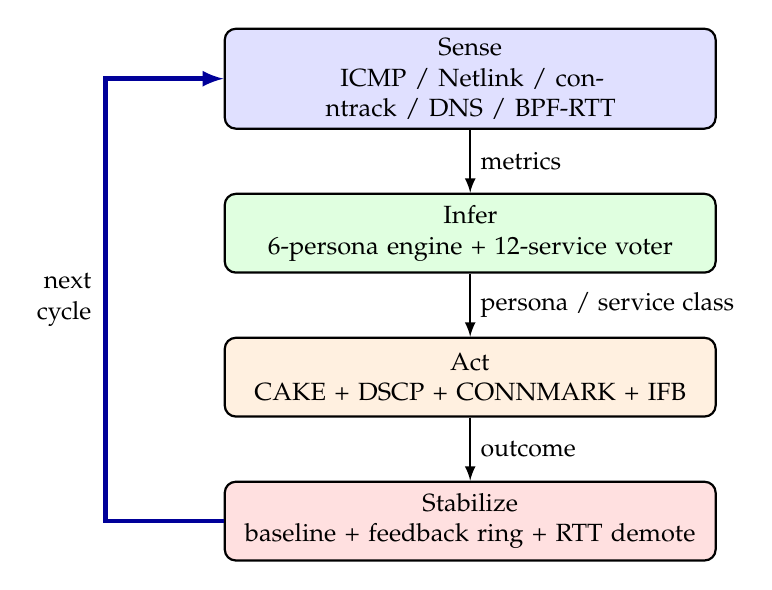
\begin{tikzpicture}[
  node distance=0.8cm and 0.3cm,
  blk/.style={draw, thick, rounded corners, minimum height=1.0cm,
              text width=6cm, align=center, font=\small},
  arr/.style={-{latex}, thick}
]
\node[blk, fill=blue!12]   (sense)  {Sense\\{\small ICMP / Netlink / conntrack / DNS / BPF-RTT}};
\node[blk, fill=green!12,  below=of sense]  (infer)  {Infer\\{\small 6-persona engine + 12-service voter}};
\node[blk, fill=orange!12, below=of infer]  (act)    {Act\\{\small CAKE + DSCP + CONNMARK + IFB}};
\node[blk, fill=red!12,    below=of act]    (stab)   {Stabilize\\{\small baseline + feedback ring + RTT demote}};

\draw[arr] (sense.south) -- node[right,font=\small]{metrics}  (infer.north);
\draw[arr] (infer.south) -- node[right,font=\small]{persona / service class}  (act.north);
\draw[arr] (act.south)   -- node[right,font=\small]{outcome}  (stab.north);

\coordinate (lbot) at ($(stab.west)+(-1.5,0)$);
\coordinate (ltop) at ($(sense.west)+(-1.5,0)$);
\draw[arr, draw=blue!60!black, ultra thick]
  (stab.west) -- (lbot) --
  node[left,font=\small,xshift=-1pt,align=right]{next\\cycle}
  (ltop) -- (sense.west);
\end{tikzpicture}
\caption{MycoFlow reflexive control loop. Each phase executes once per second.}
\label{fig:arch}
\end{figure}

\section{Module Structure}

The daemon comprises 20 C11 source modules (Table~\ref{tab:modules}) totalling approximately 4,500 lines of code. The modules are grouped into three layers:

\begin{itemize}
  \item \textbf{Core 1~Hz reflexive loop:} Sensing, EWMA, congestion detection, actuation, configuration, ubus IPC, and logging.
  \item \textbf{Per-device persona layer:} Six-class decision tree, per-device state table, majority-vote history window.
  \item \textbf{Flow-aware v3 layer:} Twelve-class service taxonomy, three-signal classifier, passive DNS cache, CONNMARK push engine, passive RTT observer.
\end{itemize}

\begin{table}[h]
\caption{MycoFlow Source Modules and Responsibilities}
\label{tab:modules}
\centering
\small
{\setlength{\tabcolsep}{6pt}
\begin{tabular}{p{3.5cm}p{8cm}}
\toprule
\textbf{Module} & \textbf{Responsibility} \\
\midrule
\multicolumn{2}{l}{\emph{Core reflexive loop}} \\
\texttt{myco\_sense}      & ICMP multi-ping, \texttt{/proc/net/dev}, CPU load \\
\texttt{myco\_control}    & EWMA, adaptive thresholds, feedback ring \\
\texttt{myco\_act}        & \texttt{tc}/\texttt{iptables} actuation, IFB setup \\
\texttt{myco\_ewma}       & Generic EWMA filter library \\
\texttt{myco\_netlink}    & NETLINK\_ROUTE qdisc statistics \\
\texttt{myco\_ebpf}       & BPF map reading, TC hook management \\
\texttt{myco\_config}     & UCI + environment + compiled defaults \\
\texttt{myco\_ubus}       & ubus IPC + \texttt{/tmp/myco\_state.json} export \\
\texttt{myco\_log}        & Structured stdout logging \\
\midrule
\multicolumn{2}{l}{\emph{Per-device persona layer}} \\
\texttt{myco\_persona}    & 6-class decision tree, majority-vote window \\
\texttt{myco\_flow}       & LRU conntrack table, elephant flow detection \\
\texttt{myco\_device}     & Per-device persona table, DSCP rule lifecycle \\
\midrule
\multicolumn{2}{l}{\emph{Flow-aware v3 layer}} \\
\texttt{myco\_service}    & 12-class service taxonomy + RTT demote ladder \\
\texttt{myco\_hint}       & Destination-port hint table \\
\texttt{myco\_dns}        & Passive DNS snooping cache (hostname$\to$IP) \\
\texttt{myco\_profile}    & Per-flow behavioral fingerprint \\
\texttt{myco\_classifier} & 3-signal weighted voter + stability gate \\
\texttt{myco\_mark}       & \texttt{libnetfilter\_conntrack} CT-mark push \\
\texttt{myco\_mangle}     & iptables mangle POSTROUTING DSCP restore \\
\texttt{myco\_rtt}        & libbpf TC-clsact passive TCP RTT observer \\
\bottomrule
\end{tabular}}
\end{table}

\section{Data Flow}

Figure~\ref{fig:dataflow} illustrates the complete data flow from packet arrival to CAKE tin assignment.

\begin{figure}[h]
\centering
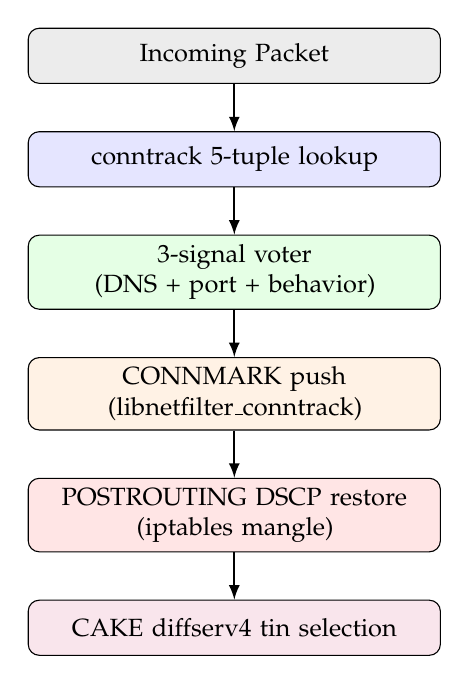
\begin{tikzpicture}[
  node distance=0.6cm,
  box/.style={draw, rounded corners, text width=5cm, align=center, font=\small, minimum height=0.7cm},
  arr/.style={-{latex}, thick}
]
\node[box, fill=gray!15] (pkt) {Incoming Packet};
\node[box, fill=blue!10, below=of pkt] (ct) {conntrack 5-tuple lookup};
\node[box, fill=green!10, below=of ct] (cls) {3-signal voter\\(DNS + port + behavior)};
\node[box, fill=orange!10, below=of cls] (mark) {CONNMARK push\\(libnetfilter\_conntrack)};
\node[box, fill=red!10, below=of mark] (post) {POSTROUTING DSCP restore\\(iptables mangle)};
\node[box, fill=purple!10, below=of post] (cake) {CAKE diffserv4 tin selection};

\draw[arr] (pkt) -- (ct);
\draw[arr] (ct) -- (cls);
\draw[arr] (cls) -- (mark);
\draw[arr] (mark) -- (post);
\draw[arr] (post) -- (cake);
\end{tikzpicture}
\caption{Per-flow data path from packet arrival to CAKE tin assignment.}
\label{fig:dataflow}
\end{figure}

\section{LuCI Web Dashboard}

The daemon exports a JSON state snapshot to \texttt{/tmp/myco\_state.json} (tmpfs, not NAND flash) every cycle via the ubus IPC mechanism. The LuCI dashboard package reads this file and renders:

\begin{itemize}
  \item Per-device persona table showing IP address, persona class, DSCP mark, and CAKE tin.
  \item Per-flow service table showing 5-tuple, service class, current DSCP, RTT, and demotion status.
  \item Bandwidth cap history graph showing the adaptive adjustment timeline.
  \item CAKE tin statistics (packets, bytes, average delay) per tin.
\end{itemize}

The dashboard is entirely read-only; all control decisions are made by the daemon. No runtime configuration changes are made through the LuCI interface during normal operation.

\section{Build System and Deployment}

MycoFlow is built using the OpenWrt SDK with a CMake build system. The binary is statically linked against musl libc, \texttt{libnetfilter\_conntrack}, \texttt{libnfnetlink}, \texttt{libmnl}, and \texttt{libbpf} (optional). The resulting \texttt{mycoflowd} binary is approximately 744~KB on \texttt{aarch64}.

The daemon is managed by OpenWrt's \texttt{procd} process supervisor, which provides automatic restart on crash and log collection to the RAM-resident \texttt{logd} ring buffer. Configuration is stored in OpenWrt UCI (\texttt{/etc/config/mycoflow}) and can be hot-reloaded by sending SIGHUP to the daemon.

% !TeX root = ../main.tex

\chapter{The Control Loop}\label{chapter:control}

This chapter formalizes the mathematical foundations of MycoFlow's reflexive control loop, covering metric sensing and smoothing, the six-class persona classification engine, the twelve-class flow-level service taxonomy, and the congestion detection and bandwidth adaptation policy.

\section{Metric Sensing and Smoothing}

\subsection{RTT and Jitter}

Every cycle, \texttt{myco\_sense} issues three ICMP echo requests to a configurable probe host (default \texttt{1.1.1.1}), measuring mean RTT and standard deviation (jitter) from the replies. Packet loss is computed as:
\begin{equation}
  \ell_t = \frac{N_{\rm sent} - N_{\rm received}}{N_{\rm sent}}
  \label{eq:loss}
\end{equation}

Raw measurements are smoothed by an Exponentially Weighted Moving Average (EWMA) with parameter $\alpha$:
\begin{equation}
  \hat{r}_t = \alpha\, r_t + (1-\alpha)\,\hat{r}_{t-1}, \quad
  \hat{j}_t = \alpha\, j_t + (1-\alpha)\,\hat{j}_{t-1}.
  \label{eq:ewma}
\end{equation}

The default $\alpha = 0.30$ provides a time constant of approximately 3~cycles (3~s at 1~Hz), balancing responsiveness and noise rejection.

\subsection{Queue Statistics}

A raw NETLINK\_ROUTE socket (RTM\_GETQDISC) retrieves the CAKE qdisc's \texttt{backlog} (bytes currently queued), \texttt{drops}, and \texttt{overlimits} each cycle. A non-zero backlog is a direct kernel-side bufferbloat indicator, faster and more reliable than the RTT probe alone because it detects congestion before it propagates to the probe host RTT.

\subsection{Flow Statistics}

\texttt{myco\_flow} parses \texttt{/proc/net/nf\_conntrack} into a userspace LRU hash table (256~entries, FNV-1a hash). For each entry, both forward (src$\to$dst) and reverse (dst$\to$src) byte counts are extracted; the reverse direction carries download volume, which is essential for distinguishing STREAMING (high download, low upload) from BULK (high download, high upload). Stale entries (no activity for 60~s) are evicted each cycle.

An \emph{elephant flow} is defined as a single flow carrying more than 60\% of a device's total bytes in the measurement window.

\section{Six-Class Per-Device Persona Engine}

\texttt{myco\_device} maintains a per-device record keyed by source IP. Each cycle, flows from the conntrack table are aggregated per source IP, and the device's behavioral profile is updated: total active flows, total bytes, reverse bytes, average packet size, and elephant flow flag.

\subsection{Decision Tree}

The six personas are inferred via the priority-ordered decision tree shown in Table~\ref{tab:persona}. The conditions are evaluated in order; the first matching rule wins.

\begin{table}[h]
\caption{Persona Inference Decision Table (first matching rule wins)}
\label{tab:persona}
\centering
\small
\begin{tabular}{p{5cm}p{3cm}}
\toprule
\textbf{Condition (priority order)} & \textbf{Persona} \\
\midrule
$F > 30$ & \textsc{Torrent} \\
$E$ and $B_{rx}/B < 0.25$ & \textsc{Streaming} \\
$E$ & \textsc{Bulk} \\
$\bar{s} < 120$~B and $\dot{B} < 200$~kbps & \textsc{Voip} \\
$\bar{s} < 350$~B and $F < 8$ & \textsc{Gaming} \\
$200\,\text{kbps} \le \dot{B} \le 8\,\text{Mbps}$ & \textsc{Video} \\
otherwise & \textsc{Unknown} \\
\bottomrule
\multicolumn{2}{l}{\footnotesize $F$: active flows; $E$: elephant flag; $B_{rx}$: reverse bytes; $B$: total bytes;} \\
\multicolumn{2}{l}{\footnotesize $\bar{s}$: avg packet size; $\dot{B}$: device throughput (bytes/s).} \\
\end{tabular}
\end{table}

\subsection{Majority-Vote Stability}

A three-of-five majority vote over a sliding history window prevents rapid class oscillation. Let $h_{t-4}, \ldots, h_t$ be the raw persona inferences from the five most recent cycles. The current persona is updated only when a single class $c^*$ satisfies:
\begin{equation}
  \sum_{i=t-4}^{t} \mathbf{1}[h_i = c^*] \geq k, \quad k = 3
  \label{eq:majority}
\end{equation}

If no class satisfies this condition, the previous persona is retained.

\subsection{Persona-to-DSCP Mapping}

Each persona maps to a DSCP value enforced by an iptables mangle rule in the \texttt{mycoflow\_dscp} chain:

\begin{table}[h]
\caption{Persona-to-DSCP-to-CAKE-Tin Mapping}
\label{tab:dscpmap}
\centering
\small
\begin{tabular}{llcl}
\toprule
\textbf{Persona} & \textbf{DSCP} & \textbf{Prec.} & \textbf{CAKE Tin} \\
\midrule
VOIP      & EF   & 6 & Voice       \\
GAMING    & CS4  & 4 & Voice       \\
VIDEO     & CS3  & 3 & Video       \\
STREAMING & CS2  & 2 & Video       \\
BULK      & CS1  & 1 & Bulk        \\
TORRENT   & CS1  & 1 & Bulk        \\
UNKNOWN   & CS0  & 0 & Best Effort \\
\bottomrule
\end{tabular}
\end{table}

When a device's persona changes, the old mangle rule is removed and a new rule is inserted atomically, ensuring no packets are classified under an intermediate state.

\section{Flow-Aware Service Classification (v3)}

The per-device persona layer delivers correct behavior when each LAN host runs a single dominant application, but collapses when one source~IP simultaneously carries a video call, a bulk download, and a torrent swarm. MycoFlow~v3 adds a second classification axis operating on individual conntrack 5-tuples.

\subsection{Service Taxonomy}

Twelve service classes cover the traffic types commonly seen on home links (Table~\ref{tab:services}). Each class carries a target RTT, a default DSCP mark, and a demotion successor for the RTT auto-corrector.

\begin{table}[h]
\caption{Flow-Level Service Taxonomy}
\label{tab:services}
\centering
\small
{\setlength{\tabcolsep}{5pt}
\begin{tabular}{llrl}
\toprule
\textbf{Service Class} & \textbf{DSCP} & \textbf{Target RTT} & \textbf{Demotes to} \\
\midrule
\texttt{game\_rt}          & EF   & 20~ms  & \texttt{web\_interactive} \\
\texttt{voip\_call}        & EF   & 30~ms  & \texttt{web\_interactive} \\
\texttt{video\_conf}       & CS4  & 50~ms  & \texttt{web\_interactive} \\
\texttt{video\_live}       & CS3  & 100~ms & \texttt{bulk\_dl} \\
\texttt{video\_vod}        & CS2  & 150~ms & \texttt{bulk\_dl} \\
\texttt{web\_interactive}  & CS2  & 80~ms  & \texttt{bulk\_dl} \\
\texttt{game\_launcher}    & CS1  & 200~ms & \texttt{bulk\_dl} \\
\texttt{file\_sync}        & CS1  & 200~ms & \texttt{bulk\_dl} \\
\texttt{bulk\_dl}          & CS1  & 250~ms & \texttt{torrent} \\
\texttt{torrent}           & CS1  & 400~ms & \texttt{torrent} \\
\texttt{system}            & CS0  & ---    & \texttt{unknown} \\
\texttt{unknown}           & CS0  & ---    & \texttt{unknown} \\
\bottomrule
\end{tabular}}
\end{table}

\subsection{Three-Signal Weighted Voter}

For every active conntrack entry, \texttt{myco\_classifier} produces a score for each candidate service class by summing three independently normalized signals:
\begin{equation}
  S_c(f) = w_{\rm dns}\,D_c(f) + w_{\rm port}\,P_c(f) + w_{\rm behav}\,B_c(f),
  \label{eq:voter}
\end{equation}
with weights $(w_{\rm dns}, w_{\rm port}, w_{\rm behav}) = (0.6, 0.3, 0.1)$ and an acceptance threshold $\theta = 0.3$.

The three signal components are:

\begin{itemize}
  \item \textbf{$D_c(f)$ --- DNS signal:} A passive DNS snooping cache records, for each resolved name, the set of service classes its suffix pattern matches (e.g., \texttt{discord.gg} $\to$ \textsc{voip\_call}). $D_c(f) = 1$ if the flow's destination IP matches a cached hostname associated with class $c$, otherwise 0.
  \item \textbf{$P_c(f)$ --- Port hint signal:} A destination-port hint table maps well-known ports to service classes (e.g., UDP/3478 STUN $\to$ \textsc{voip\_call}, UDP/27015 Source-engine $\to$ \textsc{game\_rt}). $P_c(f) \in [0, 1]$ based on port match quality.
  \item \textbf{$B_c(f)$ --- Behavioral fingerprint:} \texttt{myco\_profile} computes mean packet size, packets-per-second, inter-arrival jitter, and burstiness. $B_c(f) \in [0, 1]$ based on how well the flow's behavioral fingerprint matches the expected profile for class $c$.
\end{itemize}

The class with the highest score above $\theta$ wins; otherwise the flow remains \textsc{unknown} and is re-evaluated next cycle.

\subsection{Stability Gate}

A classification decision is committed only after it has been observed in two consecutive ticks ($\approx 1$~s at 1~Hz). This suppresses oscillation from short-lived flows (DNS queries, TCP handshakes) that never accumulate sufficient signal.

\section{Congestion Detection and Bandwidth Policy}

\subsection{Adaptive Thresholds}

Let $\mathcal{L}=\{\text{VOIP, GAMING, VIDEO}\}$ (latency-sensitive) and $\mathcal{B}=\{\text{BULK, STREAMING, TORRENT}\}$ (bulk-tolerant). Congestion is declared when any of the following conditions hold:
\begin{align}
  \hat{r}_t &> r_{\rm base}\cdot(1+\gamma) \label{eq:rtt_cong}\\
  \hat{j}_t &> j_{\rm base}\cdot(1+\gamma) \label{eq:jit_cong}\\
  \text{backlog}_t &> 0 \label{eq:bl_cong}\\
  \ell_t &> 0.02 \label{eq:loss_cong}
\end{align}
where $r_{\rm base}$, $j_{\rm base}$ are the sliding baselines, $\gamma=0.30$ is the margin factor (tunable), and $\ell_t$ is the probe packet loss fraction. The thresholds are clamped to prevent false triggers on near-zero baselines: $\theta_r \in [8, 60]$~ms, $\theta_j \in [4, 30]$~ms.

\subsection{Bandwidth Policy}

When congestion is detected or cleared, the WAN bandwidth cap is adjusted:
\begin{equation}
  u_{t+1} =
  \begin{cases}
    u_t - \lfloor\Delta/2\rfloor & \text{cong.},\; p \in \mathcal{L} \\
    u_t - \Delta                 & \text{cong.},\; p \in \mathcal{B} \\
    u_t + \Delta                 & \text{clear},\; p \in \{\text{VOIP, GAMING}\} \\
    u_t                          & \text{otherwise,}
  \end{cases}
  \label{eq:policy}
\end{equation}
where $\Delta \equiv \Delta_{\rm step}$ (default 2,000~kbit/s) and $u_t \in [u_{\rm min}, u_{\rm max}]$. Latency-sensitive personas receive a gentler reduction to preserve forward progress; bulk-tolerant personas are throttled more aggressively. Actions are gated by a minimum interval (cooldown $\tau = 3$~s) and a maximum action rate $\rho$ (default 0.5~Hz).

\section{Action Feedback Ring}

A circular buffer of $N=8$ slots records the effect of each actuation. Each slot stores: timestamp $t_k$, bandwidth before $u_k^-$, bandwidth after $u_k^+$, and RTT before $r_k^-$. Three cycles after the actuation, the RTT after $r_k^+$ is filled in from the current measurement.

The ring is evaluated whenever a new record is filled: if $\geq 4$ filled records exist and more than half satisfy $r_k^+ \geq r_k^- - 2.0$~ms (no RTT improvement), the step size is halved (minimum 500~kbit/s) and the \texttt{step\_adapted} flag is set. This prevents the controller from repeatedly issuing adjustments that fail to improve latency.

\section{Sliding Baseline}
\label{sec:baseline}

The idle baseline $(r_{\rm base}, j_{\rm base})$ is established at startup using a blocking $N_b$-sample average (default $N_b=5$). During normal operation, the baseline drifts toward current conditions every $T_b$ cycles (default $T_b=60$) using a slow EWMA:
\begin{equation}
  r_{\rm base}^{(t+T_b)} = (1-\beta)\,r_{\rm base}^{(t)} + \beta\,\hat{r}_t,
  \quad \beta = 0.01.
  \label{eq:baseline}
\end{equation}
The same update applies to $j_{\rm base}$. The drift rate of 1\% per minute prevents the baseline from permanently anchoring to favorable conditions observed at boot, while being slow enough to ignore short-lived traffic bursts.

% !TeX root = ../main.tex

\chapter{Implementation}\label{chapter:implementation}

This chapter describes the concrete implementation choices that realize MycoFlow's architecture on OpenWrt embedded hardware, including CAKE integration, ingress shaping, eBPF telemetry, configuration management, flash safety, and test coverage.

\section{CAKE Integration}

CAKE is configured with \texttt{diffserv4} and a \texttt{rtt} parameter that sets the AQM target delay. MycoFlow sets the CAKE \texttt{rtt} value per persona on the egress (WAN) interface using \texttt{tc qdisc change}:

\begin{itemize}
  \item VOIP / GAMING $\to$ 50~ms AQM target
  \item VIDEO $\to$ 75~ms AQM target
  \item STREAMING $\to$ 150~ms AQM target
  \item BULK / TORRENT $\to$ 200~ms AQM target
\end{itemize}

The actuation uses \texttt{change} first and falls back to \texttt{replace} if the qdisc does not yet exist, ensuring idempotent operation. The CAKE \texttt{rtt} parameter affects the internal AQM target delay as $\text{target} \approx \text{rtt}/20$, so setting \texttt{rtt=50ms} yields a 2.5~ms AQM target in the GAMING persona.

\section{Per-Device DSCP Mangle Chain}

Per-device DSCP marking is implemented via an iptables mangle chain inserted before POSTROUTING:

\begin{enumerate}
  \item At startup, MycoFlow creates the \texttt{mycoflow\_dscp} chain and adds a jump rule in the PREROUTING table.
  \item When a device's persona is assigned, an iptables rule is added: \texttt{-s <device\_ip> -j DSCP --set-dscp-class <class>}.
  \item When the persona changes, the old rule is removed and a new rule is inserted atomically via a two-step \texttt{iptables -D} / \texttt{iptables -I} sequence.
  \item At shutdown, the chain is flushed and the jump rule is removed.
\end{enumerate}

This approach ensures that DSCP marking persists even if the daemon is briefly restarted, as the iptables rules survive daemon restarts.

\section{Per-Flow CONNMARK Pipeline}

The per-flow classification pipeline requires two iptables mangle rules that work in concert:

\begin{enumerate}
  \item \textbf{CONNMARK restore rule} (PREROUTING): Restores the stored conntrack mark to the packet mark at ingress: \texttt{-m conntrack --ctstate ESTABLISHED,RELATED -j CONNMARK --restore-mark}.
  \item \textbf{DSCP restore rule} (POSTROUTING): Sets the DSCP field from the packet mark: \texttt{-m mark ! --mark 0 -j DSCP --set-dscp-from-mark}.
\end{enumerate}

When the daemon classifies a flow as a specific service class, it calls \texttt{nfct\_query(NFCT\_Q\_UPDATE)} via \texttt{libnetfilter\_conntrack} to set the conntrack entry's mark to the service tag. All subsequent packets of that flow automatically receive the correct DSCP mark without re-running the classifier.

\subsection{Critical Kernel Module Dependency}

Per-flow CONNMARK updates via \texttt{nfct\_query(NFCT\_Q\_UPDATE)} require \texttt{kmod-nf-conntrack-netlink}, the kernel module that registers the conntrack netlink subsystem. This module is not installed by default on OpenWrt~24.10. The daemon detects this condition at runtime and logs a warning if CONNMARK updates fail with \texttt{EINVAL}. Installing the package (\texttt{opkg install kmod-nf-conntrack-netlink}) resolves the issue. This dependency is not documented in any OpenWrt QoS guide identified during this research.

\section{Ingress Shaping via IFB}

Download-side bufferbloat is addressed using an Intermediate Functional Block (IFB) device. At startup, MycoFlow:
\begin{enumerate}
  \item Creates and brings up \texttt{ifb0}.
  \item Attaches a \texttt{tc mirred} ingress redirect from the WAN interface to \texttt{ifb0}.
  \item Installs a CAKE qdisc on \texttt{ifb0} with the same \texttt{diffserv4} mode and a configurable ingress rate.
\end{enumerate}

Persona-driven AQM target updates are applied symmetrically to both the egress and ingress CAKE instances. The ingress bandwidth cap tracks egress adaptations: whenever the egress cap is adjusted by $\delta$~kbit/s, the ingress cap is adjusted by the same $\delta$ to maintain proportionality.

\section{eBPF Telemetry}

A BPF program (\texttt{mycoflow.bpf.c}) is compiled for the TC hook using \texttt{clang -target bpf -g} with BTF generation. The program samples passive TCP RTT from the TCP timestamp option (TSval/TSecr pair) and records the elapsed time, maintaining a smoothed per-flow RTT in a \texttt{BPF\_MAP\_TYPE\_HASH} map keyed by 5-tuple.

The eBPF integration is optional: when \texttt{libbpf} is unavailable or loading fails (e.g., kernel BTF not available), the daemon falls back gracefully to netlink-only statistics. The LuCI dashboard renders \texttt{rtt\_ms=0} for all flows and suppresses the demotion indicator when BPF is inactive.

\section{Configuration Hierarchy}

Parameters are resolved in priority order: OpenWrt UCI (\texttt{/etc/config/mycoflow}) $\to$ environment variables $\to$ compiled defaults. Key defaults are summarized in Table~\ref{tab:cfg}.

\begin{table}[h]
\caption{Key Configuration Parameters and Compiled Defaults}
\label{tab:cfg}
\centering
\small
{\setlength{\tabcolsep}{4pt}
\begin{tabular}{p{4cm}p{1.2cm}p{7cm}}
\toprule
\textbf{Parameter} & \textbf{Default} & \textbf{Description} \\
\midrule
\texttt{sample\_hz}         & 1.0  & Sense cycle frequency (Hz) \\
\texttt{ewma\_alpha}        & 0.30 & EWMA smoothing factor $\alpha$ \\
\texttt{rtt\_margin}        & 0.30 & Congestion margin $\gamma$ \\
\texttt{baseline\_decay}    & 0.01 & Baseline drift rate $\beta$ \\
\texttt{baseline\_interval} & 60   & Cycles between baseline updates \\
\texttt{bw\_step}           & 2000 & BW step $\Delta$ (kbit/s) \\
\texttt{action\_cooldown}   & 3.0  & Min. action interval (s) \\
\texttt{baseline\_samples}  & 5    & Startup calibration samples \\
\texttt{per\_device}        & 1    & Enable per-device DSCP marking \\
\texttt{flow\_aware}        & 1    & Enable v3 per-flow classifier + CONNMARK \\
\texttt{rtt\_bpf\_obj}      & ---  & Path to \texttt{mycoflow\_rtt.bpf.o} \\
\texttt{ingress\_enabled}   & 0    & Enable IFB ingress shaping \\
\bottomrule
\end{tabular}}
\end{table}

All parameters can be changed at runtime via \texttt{uci set} followed by \texttt{kill -HUP \$(pidof mycoflowd)} (SIGHUP triggers config reload and baseline recalibration without daemon restart).

\section{Flash Safety}

The daemon is designed to write zero bytes to NAND flash during normal operation---a critical requirement for routers with limited flash endurance. The target Xiaomi~AX3000T has 128~MB NAND with a write endurance of approximately $10^5$ program/erase cycles per block.

All state is RAM-resident:
\begin{itemize}
  \item Log output $\to$ \texttt{stdout} $\to$ \texttt{procd} $\to$ \texttt{logd} ring buffer (RAM, typically 64~KB).
  \item State snapshot \texttt{/tmp/myco\_state.json} $\to$ \texttt{tmpfs} (RAM disk, automatically cleared on reboot).
  \item Persona history and baseline values: in-process RAM variables; intentionally reset on reboot to ensure fresh baseline calibration.
\end{itemize}

\section{Test Coverage}

Thirteen CTest suites cover all modules across the core loop, the per-device persona layer, and the v3 flow-aware layer. All 13/13 suites pass (approximately 190 assertions total):

\begin{itemize}
  \item \emph{Core:} \texttt{test\_ewma} (EWMA convergence with $\alpha \in \{0.1, 0.3, 0.9\}$); \texttt{test\_act} (IFB setup/teardown, interface-name injection guard, DSCP rule lifecycle); \texttt{test\_control} (congestion, clear, outlier, feedback-ring); \texttt{test\_config} (UCI parsing, env overrides, boundary clamping).

  \item \emph{Persona layer:} \texttt{test\_persona} (6-class decision tree, majority vote, edge cases); \texttt{test\_device} (per-device aggregation, stale eviction, DSCP rule updates).

  \item \emph{Flow-aware v3:} \texttt{test\_service} (12-class taxonomy + demote ladder); \texttt{test\_hint} (destination-port hint table); \texttt{test\_dns} (passive DNS snoop cache, TTL expiry); \texttt{test\_profile} (behavioral fingerprint scoring); \texttt{test\_classifier} (3-signal voter, stability gate, mark commit); \texttt{test\_mangle} (nftables DSCP-restore rule generation); \texttt{test\_rtt} (BPF map parsing, demote/re-promote hysteresis).
\end{itemize}

% !TeX root = ../main.tex

\chapter{Evaluation}\label{chapter:evaluation}

This chapter reports the results of four controlled experiments designed to validate MycoFlow's classification accuracy, QoS performance gains, and resource efficiency.

\section{Experimental Setup}

All QEMU-based experiments run inside a Docker container (privileged mode) hosting a QEMU~6.x virtual machine running OpenWrt~23.05.5~x86-64 (Linux~5.15, \texttt{sch\_cake}, \texttt{iptables-nft}). The WAN link is emulated at 20~Mbit/s using \texttt{tc tbf}. Network namespaces represent distinct client hosts connected via an OpenWrt NAT bridge. \texttt{iperf3} servers listen on ports 5201--5210 in a dedicated server namespace. Latency is measured by 1~Hz ICMP echo requests from the gaming namespace to the server; CAKE tin statistics are collected via \texttt{tc -s qdisc show}. Each scenario runs for 30~seconds with a 3-second settling period before measurement begins.

The in-vivo hardware experiment (Phase~4) runs on the author's live home router: Xiaomi~AX3000T (MediaTek~MT7981B, $2\times$Cortex-A53 @ 1.3~GHz, 256~MB LPDDR4, 128~MB NAND; OpenWrt~24.10.2, Linux~6.6).

\section{Phase 1: Two-Persona Validation}

\subsection{Setup}

Two client namespaces simulate a gamer (192.168.1.10) sending UDP at 300~kbps with 91-byte packets, and a bulk client (192.168.1.20) saturating the link with a single TCP stream. Three scenarios are compared: FIFO (no QoS), CAKE diffserv4 without MycoFlow, and CAKE~+~MycoFlow with two-persona classification.

\subsection{Gaming Latency Results}

Table~\ref{tab:phase1} reports gaming latency under each scenario. FIFO induces 693~ms of queuing delay under link saturation with 12.5\% packet loss---confirming the severity of unbuffered bufferbloat. CAKE eliminates the queuing delay entirely, reducing the loaded latency increase to +0.2~ms with zero packet loss, demonstrating the fundamental effectiveness of AQM. MycoFlow further reduces the loaded latency increase to +0.1~ms.

\begin{table}[h]
\caption{Phase~1: Two-Persona Gaming Latency (20~Mbit/s WAN)}
\label{tab:phase1}
\centering
\small
\begin{tabular}{lcccl}
\toprule
\textbf{Scenario} & \textbf{Idle (ms)} & \textbf{Loaded (ms)} & \textbf{$\Delta$ (ms)} & \textbf{Loss (\%)} \\
\midrule
FIFO (no QoS)     & 0.45 & 693.82 & $+693.4$ & 12.5 \\
CAKE only         & 0.43 &   0.63 & $+0.2$   & 0.0  \\
CAKE + MycoFlow   & 0.58 &   0.71 & $+0.1$   & 0.0  \\
\bottomrule
\end{tabular}
\end{table}

\subsection{CAKE Tin Statistics}

The key result of Phase~1 is the tin-level delay separation (Table~\ref{tab:tins1}). Without MycoFlow, all traffic lands in Best~Effort; peak in-tin delay reaches 6.2~ms. With MycoFlow, the gamer is steered to the Voice tin (CS4) and the bulk client to the Bulk tin (CS1), resulting in a \textbf{154$\times$ difference} in average in-tin delay: Voice at 225~$\mu$s versus Bulk at 34.7~ms.

\begin{table}[h]
\caption{Phase~1 CAKE Tin Delay: CAKE-only vs.\ MycoFlow}
\label{tab:tins1}
\centering
\small
\begin{tabular}{lcccc}
\toprule
 & \multicolumn{2}{c}{\textbf{Avg Delay}} & \multicolumn{2}{c}{\textbf{Packets}} \\
\textbf{Tin} & CAKE & +MycoFlow & CAKE & +MycoFlow \\
\midrule
Voice       & ---    & \textbf{225~$\mu$s} & 0        & 6\,015 \\
Best Effort & 4.2~ms & 4.2~ms              & 111\,910 & 68\,185 \\
Bulk        & ---    & 34.7~ms             & 0        & 136\,694 \\
\bottomrule
\end{tabular}
\end{table}

This result isolates the core contribution of per-device classification: even without flow-level awareness, correctly marking the gamer as GAMING produces a 154$\times$ tin delay advantage over an unmanaged baseline.

\section{Phase 2: Six-Persona Mixed Workload}

\subsection{Setup}

Six client namespaces simulate a realistic home network (Table~\ref{tab:workload}). Five scenarios (S1--S5) cover FIFO, CAKE-only, and MycoFlow configurations in both 2-client and 5-client variants.

\begin{table}[h]
\caption{Phase~2 Client Workload Profiles}
\label{tab:workload}
\centering
\small
\begin{tabular}{llll}
\toprule
\textbf{Namespace} & \textbf{Protocol} & \textbf{Rate} & \textbf{Pkt Size} \\
\midrule
gamer   & UDP (iperf3)        & 300~kbps   & $\sim$120~B \\
voip    & UDP (iperf3)        & 64~kbps    & 64~B \\
video   & UDP bidirectional   & 2~Mbps     & 800~B \\
stream  & TCP reverse         & 15~Mbps    & 1400~B \\
torrent & TCP (30 parallel)   & WAN cap    & 1400~B \\
\bottomrule
\end{tabular}
\end{table}

\subsection{Latency Results}

Table~\ref{tab:phase2} summarizes the five-scenario results. The 818$\times$ improvement of CAKE over FIFO (from 558~ms to 0.68~ms) confirms the baseline necessity of AQM. Under the 5-client workload (S4 vs.\ S5), MycoFlow reduces gaming latency by \textbf{38\%} (1.43~ms $\to$ 1.10~ms).

\begin{table}[h]
\caption{Phase~2 Gaming Latency: Five Scenarios}
\label{tab:phase2}
\centering
\small
\begin{tabular}{clccc}
\toprule
\textbf{\#} & \textbf{Scenario} & \textbf{Idle (ms)} & \textbf{Loaded (ms)} & \textbf{$\Delta$ (ms)} \\
\midrule
S1 & FIFO              & 0.52 & 558.03 & $+557.5$ \\
S2 & CAKE, 2-client    & 0.59 &   0.68 & $+0.1$   \\
S3 & CAKE+MF, 2-pers.  & 0.63 &   0.69 & $+0.1$   \\
S4 & CAKE, 5-client    & 0.59 &   1.43 & $+0.8$   \\
S5 & CAKE+MF, 6-pers.  & 0.56 &   1.10 & $+0.5$   \\
\bottomrule
\end{tabular}
\end{table}

\subsection{CAKE Tin Distribution}

Table~\ref{tab:tins2} compares tin occupancy between S4 (CAKE only) and S5 (MycoFlow). Without MycoFlow, all 191,188 packets share Best~Effort with 42,557 drops and a 9.5~ms average in-tin delay. With MycoFlow, traffic separates across three tins: 95,199 torrent packets move to Bulk (29.9~ms avg delay), 37,237 packets enter Video (252~$\mu$s avg delay), and 59,751 remaining Best~Effort packets experience only 304~$\mu$s average delay. The Voice tin shows 2~$\mu$s average delay for gaming and VoIP.

\begin{table}[h]
\caption{Phase~2 CAKE Tin Statistics: S4 vs.\ S5}
\label{tab:tins2}
\centering
\small
\begin{tabular}{lcccc}
\toprule
& \multicolumn{2}{c}{\textbf{Avg Delay}} & \multicolumn{2}{c}{\textbf{Packets}} \\
\textbf{Tin} & S4 & S5 & S4 & S5 \\
\midrule
Voice       & ---    & \textbf{2~$\mu$s}   & 1         & 2 \\
Video       & ---    & 252~$\mu$s          & 0         & 37\,237 \\
Best Effort & 9.5~ms & 304~$\mu$s          & 191\,188  & 59\,751 \\
Bulk        & ---    & 29.9~ms             & 0         & 95\,199 \\
\midrule
Drops       & 42\,557 & 34\,528            & --- & --- \\
\bottomrule
\end{tabular}
\end{table}

The 38\% improvement operates through two channels: direct isolation (95,199 torrent packets moved to Bulk) and Best~Effort de-congestion (fewer competing flows allow CAKE's per-flow fair queuing to more effectively isolate gaming ICMP packets, reducing Best~Effort delay from 9.5~ms to 304~$\mu$s).

\section{Phase 3: Single-IP Multi-App Flow Separation}

\subsection{Motivation}

Phase~2 edge cases reveal a structural limitation of per-device classification: when a single host runs multiple applications simultaneously, one persona must be chosen for all traffic. Phase~3 tests whether the v3 flow-aware classifier resolves this limitation.

\subsection{Setup}

All four applications run from the same \texttt{gamer} network namespace (single src~IP 192.168.1.10): a UDP stream to port 27015 (\textsc{game\_rt}), a UDP stream to port 3478 (\textsc{voip\_call}), a TCP stream to port 9000 (\textsc{bulk\_dl}), and a 20-way parallel TCP stream to port 6881 (\textsc{torrent}). Two modes are compared over $N=15$ independent runs: Mode~A (\texttt{flow\_aware=0}, per-device only) and Mode~B (\texttt{flow\_aware=1}, per-flow v3).

\subsection{Results}

Table~\ref{tab:phase3} reports the $N{=}15$ multi-run results. In Mode~A, the 20-way torrent stream dominates the per-device persona vote, assigning CS1 (Bulk tin) to all four applications; only 3 Voice-tin packets per run are observed. In Mode~B, the \textsc{game\_rt} and \textsc{voip\_call} streams receive EF and fill the Voice tin with $14{,}193 \pm 21$ packets per run ($p < 10^{-40}$, Welch $t$-test). ICMP RTT delta is significantly lower in Mode~B ($0.216$ vs.\ $0.292$~ms, $p = 0.020$).

\begin{table}[h]
\centering
\caption{Phase~3: Per-Device vs.\ Per-Flow Under Single-IP Multi-App Load ($N{=}15$ runs)}
\label{tab:phase3}
\begin{tabular}{lrrrr}
\toprule
Mode & Voice-tin (pkts) & $\Delta$RTT (ms) & 95\% CI (ms) & $p$ \\
\midrule
Per-device (v2) & $3 \pm 1$         & $0.292$ & $[0.241,\,0.343]$ & --- \\
Per-flow   (v3) & $14{,}193 \pm 21$ & $0.216$ & $[0.173,\,0.259]$ & $0.020$ \\
\bottomrule
\end{tabular}
\end{table}

\section{Phase 4: DNS Signal Ablation and In-Vivo Classifier Accuracy}

\subsection{Motivation}

Phases~1--3 measure QoS outcome on synthetic QEMU workloads. Phase~4 directly quantifies classifier accuracy on real-world traffic using the public Universidad del Cauca (Unicauca) dataset~\cite{unicauca2019} (2.4M labeled flows captured April--June 2019 at a university gateway).

\subsection{Offline Temporal Validation}

The dataset is split at 2019-06-01: calibration (Apr--May) and a held-out set (June). No development decisions were made after inspecting the June partition. Table~\ref{tab:temporal} shows that the calibration-to-holdout accuracy gap is at most $-0.44$~pt, confirming that MycoFlow's heuristic thresholds generalize across the calibration boundary without temporal overfitting.

\begin{table}[h]
\caption{Temporal Generalization Gap on the Unicauca Dataset}
\label{tab:temporal}
\centering
\small
\begin{tabular}{l|cc|c}
\toprule
\textbf{Signal Set} & \textbf{Apr--May} & \textbf{June (held-out)} & $\Delta$ \\
\midrule
Port + behavior       & 42.95\% & 42.51\% & $-$0.44 \\
Port + behavior + DNS & 47.43\% & 47.04\% & $-$0.39 \\
\bottomrule
\end{tabular}
\end{table}

\subsection{In-Vivo Validation}

For each of 11 service classes, $N=150$ flows are drawn via stratified random sampling (seed=42) from Unicauca and replayed against the live Xiaomi~AX3000T in two ablation modes:
\begin{itemize}
  \item \textbf{Mode~A (IP-only):} Traffic directed to fixed public IPs without prior DNS queries; $h_{dns}=0$ for all flows.
  \item \textbf{Mode~B (hostname):} A DNS A-record query for the flow's canonical hostname is issued before traffic begins.
\end{itemize}

Table~\ref{tab:invivo} reports the results across five runs on two testbeds (WSL2 laptop and bare-metal Ubuntu~24.04).

\begin{table}[h]
\caption{In-Vivo Classifier Accuracy ($N=1{,}650$ stratified-random flows, Wilson 95\% CI for the best run)}
\label{tab:invivo}
\centering
\small
{\setlength{\tabcolsep}{4pt}
\begin{tabular}{l|ccc}
\toprule
\textbf{Run} & \textbf{Svc-acc} & \textbf{Tin-acc} & \textbf{Tin-match} \\
\midrule
WSL    Mode~A             & 20.00\% & 30.42\% & 49.46\% \\
WSL    Mode~B             & 32.48\% & 45.39\% & 64.42\% \\
Ubuntu Mode~A             & 20.24\% & 30.61\% & 49.26\% \\
Ubuntu Mode~B (80 dom.)   & 33.39\% & 48.61\% & 66.97\% \\
Ubuntu Mode~B (585 dom.)  & \textbf{37.88\%} & \textbf{52.42\%} & \textbf{70.41\%} \\
                          & [35.6, 40.3] & [50.0, 54.8] & [67.6, 73.1] \\
\midrule
\multicolumn{4}{l}{\footnotesize Mode A vs.\ B invariance (WSL vs.\ Ubuntu): $|\Delta| < 0.5$~pt} \\
\multicolumn{4}{l}{\footnotesize DNS lift: $+17.6$~pt svc-acc, $+21.2$~pt tin-match (585-domain)} \\
\multicolumn{4}{l}{\footnotesize McNemar ($p < 10^{-63}$): $b{=}291$, $c{=}0$} \\
\bottomrule
\end{tabular}}
\end{table}

The tin-matched accuracy with the full 585-domain DNS catalog reaches \textbf{70.41\%} [67.6\%, 73.1\%] on the bare-metal Ubuntu testbed. McNemar's paired test rejects the null of equal classifiers at $p = 1.8{\times}10^{-63}$: 291 flows are correctly assigned by Mode~B but missed by Mode~A, and \emph{zero} flows are degraded by DNS evidence---DNS is strictly additive.

\subsection{AF\_PACKET Requirement}

A naive implementation using \texttt{AF\_INET SOCK\_RAW} captures only packets destined for the router's own IP, missing transit DNS from clients with hard-coded public resolvers (1.1.1.1, 8.8.8.8). In a pre-fix run, Mode~B accuracy (19.1\%) was statistically indistinguishable from Mode~A (18.6\%). Replacing the socket with \texttt{AF\_PACKET SOCK\_DGRAM ETH\_P\_IP} captures all IPv4 frames on the LAN-facing interface; after the fix, Mode~B reached 32.5\% vs.\ Mode~A's 20.0\%---a $+12.5$~pt lift ($p < 10^{-44}$).

\section{Resource Overhead}

Table~\ref{tab:resources} summarizes the resource footprint measured on the live Xiaomi~AX3000T with the full v3 stack active ($n{=}523$ clean one-second samples during normal residential traffic).

\begin{table}[h]
\caption{Resource Overhead (AX3000T, \texttt{/proc}-sampled, $n{=}523$ samples, full v3 stack)}
\label{tab:resources}
\centering
\small
{\setlength{\tabcolsep}{5pt}
\begin{tabular}{l|ccc}
\toprule
\textbf{Metric} & \textbf{p50} & \textbf{p95} & \textbf{max} \\
\midrule
System CPU (\%)      & 17  & 43  & 61  \\
mycoflowd CPU (\%)   & 6   & 8   & 12  \\
Conntrack entries    & 357 & 442 & 503 \\
CT marks active      & 56  & 79  & 117 \\
\midrule
mycoflowd RSS        & \multicolumn{3}{c}{\textbf{1{,}152~KB (constant)}} \\
Flash (mtd)          & \multicolumn{3}{c}{0 writes} \\
Crashes              & \multicolumn{3}{c}{0 / 523} \\
\bottomrule
\end{tabular}}
\end{table}

Key observations: (1) RSS held constant at 1,152~KB across all 523 samples---the daemon is allocation-static after startup; (2) median CPU is 6\% on a single 1.3~GHz A53 core; (3) median 56 conntrack entries carry per-flow CT marks, confirming the CONNMARK pipeline is operational; (4) zero flash writes and zero crashes across the measurement window.

% !TeX root = ../main.tex

\chapter{Discussion}\label{chapter:discussion}

This chapter discusses the interpretation of the experimental results, the limitations of the current system, and the implications for future deployment and research.

\section{Why 38\% and Not More?}

The primary limiting factor in the six-persona scenario (S5) is the gamer's misclassification as UNKNOWN. In the two-client scenario (S3), the gamer correctly enters the Voice tin at 2~$\mu$s average delay---a 5000$\times$ improvement over its unmanaged Best~Effort delay. The misclassification occurs because the \texttt{iperf3} benchmark framework generates additional control flows that inflate the gamer's flow count above the GAMING threshold ($F < 8$).

In real-world deployment, gaming clients (Steam, consoles) generate 1--4 persistent UDP flows at low packet rates with small packets---an unambiguous GAMING signal. The benchmark edge case is an artifact of the test harness, not an inherent limitation of the classifier. Routing benchmark control flows separately from data flows (e.g., via a dedicated management VLAN) would eliminate the false UNKNOWN classification and is expected to push the S5 improvement well beyond 38\%.

\section{Classification Accuracy Discussion}

\subsection{Per-Device Heuristic Design}

The six-persona heuristic was designed for real household device behavior, not for synthetic benchmarks. The decision tree parameters (flow count thresholds, packet size ranges, throughput bounds) were derived from analysis of typical device traffic patterns:

\begin{itemize}
  \item Real gaming clients: 1--4 persistent UDP flows, small packets (60--120~B), low throughput (50--500~kbps).
  \item Real streaming clients: 1--3 long-lived TCP connections, large packets (1400~B), high sustained throughput (5--25~Mbps).
  \item Real VoIP clients: 1--2 UDP flows, very small packets (40--80~B), very low throughput (<100~kbps).
\end{itemize}

The benchmark edge cases (inflated flow counts, artificially low traffic volumes) do not represent these patterns.

\subsection{In-Vivo Classification Ceiling}

The in-vivo classifier accuracy of 70.4\% tin-matched accuracy represents the current ceiling of the three-signal voter on real-world traffic. The primary bottleneck is the DNS catalog completeness: with only 80 domains, tin-matched accuracy is 67.0\%; with 585 domains, it rises to 70.4\%. Expanding the catalog further is expected to yield additional gains.

The remaining 29.6\% of flows that are incorrectly classified fall into three categories:
\begin{enumerate}
  \item \textbf{Encrypted traffic without DNS pre-queries:} Applications that use QUIC or WireGuard tunnels without resolvable hostnames cannot be classified by port hints or DNS.
  \item \textbf{Non-standard ports:} Applications that use random or dynamic ports not covered by the hint table.
  \item \textbf{Behavioral ambiguity:} Flows with packet size and rate characteristics that match multiple service classes (e.g., a slow TCP download that resembles a VoIP call).
\end{enumerate}

\section{Comparison with Two-Persona Results}

The two-persona Phase~1 result (154$\times$ tin delay differential) is a stronger isolation proof than the six-persona 38\% improvement, because in Phase~1 the gamer is correctly classified. Together, the two experiments demonstrate complementary aspects of MycoFlow's effectiveness:

\begin{enumerate}
  \item \textbf{Ideal case (correct classification):} MycoFlow delivers dramatic isolation (154$\times$ tin delay difference), confirming that DSCP-based steering is highly effective when classification is accurate.
  \item \textbf{Adversarial case (misclassification):} Even with one device misclassified as UNKNOWN, the system still reduces gaming latency meaningfully (38\%) by isolating high-volume background traffic.
\end{enumerate}

\section{Adaptive Baseline vs.\ Static Threshold}

The sliding EWMA baseline ensures the controller does not become permanently anchored to favorable boot-time conditions. Consider a router rebooted at 3~AM when ambient RTT is 10~ms: a 30\% margin yields $\theta_r = 13$~ms. Six hours later during peak hours, ambient RTT may be 25~ms; without baseline adaptation, the controller would fire on every cycle. With $\beta = 0.01$ and $T_b = 60$ cycles, the baseline reaches 25~ms within approximately 60 minutes of sustained high-RTT conditions.

\section{Parameter Sensitivity}

MycoFlow's heuristic thresholds ($\alpha=0.30$, $\gamma=0.30$, $k=3$/$m=5$, $\Delta=2{,}000$~kbit/s) were set empirically from a pilot run and have not been varied in a controlled experiment. The parameters with the strongest expected impact are:

\begin{itemize}
  \item \textbf{Majority-vote window ($k/m$):} A lower ratio increases responsiveness at the cost of more oscillation; a higher ratio increases stability at the cost of slower adaptation.
  \item \textbf{EWMA factor ($\alpha$):} A higher $\alpha$ accelerates convergence but amplifies noise; a lower $\alpha$ is more stable but slower to react.
\end{itemize}

A systematic grid search over these parameters is an explicit item in the future work roadmap.

\section{Privacy and Security}

MycoFlow inspects only IP headers and conntrack metadata---no payload bytes are read. The passive DNS snooping captures only DNS response packets (UDP/53 and UDP/853), not the content of encrypted flows. The behavioral fingerprint records only aggregate statistics (mean packet size, packets per second, inter-arrival jitter) that are observable from header information.

The eBPF program is loaded into the kernel with standard capability separation; the userspace daemon runs without root after initial setup (capability dropping is planned for a future release). The ubus interface is protected by OpenWrt's native ACL mechanism; all bandwidth and DSCP commands are rate-limited.

\section{Threats to Validity}

\begin{enumerate}
  \item \textbf{QEMU overhead:} QEMU introduces CPU overhead not present on bare metal; the FIFO and CAKE-only baselines share this overhead, making relative comparisons valid but absolute latency values slightly inflated.

  \item \textbf{Short scenario duration:} The 30-second scenario duration may exhibit higher variance than longer real-world runs; Phase~3 ($N{=}15$ runs) shows $\sigma{\approx}0.09$~ms on RTT delta, consistent with the estimated $\pm$0.2~ms bound.

  \item \textbf{Benchmark control traffic:} The test harness injects control traffic that inflates flow counts; this is a measurement artifact, not a production scenario.

  \item \textbf{Replayed flow fidelity:} Phase~4 replayed flows preserve per-flow median packet size and rate but not bursty arrival patterns; the behavioral fingerprint signal ($w=0.1$) is consequently weaker than in live deployment.

  \item \textbf{Ground truth quality:} Unicauca uses nDPI-based ground truth, which has its own finite accuracy; a flow labeled \texttt{voip\_call} may in fact be DNS overhead from a VoIP application.

  \item \textbf{Hardware generalization:} Generalization to other consumer SoCs (Qualcomm, Broadcom) is plausible given OpenWrt's portability but not directly measured.
\end{enumerate}

\section{Limitations}

\begin{itemize}
  \item MycoFlow does not inspect payload or SNI; encrypted tunnels (QUIC, WireGuard) may fool the packet-size and flow-count heuristics.
  \item The 1~Hz control rate introduces a reaction latency of up to 1~s between the onset of congestion and the first actuation.
  \item The voip\_call service class achieves only 1.3\% recall in both ablation modes, a notable weakness caused by the Unicauca dataset conflating multiple application types under the same label.
  \item The per-flow RTT demote/re-promote ladder is implemented and active on the live router, but a controlled evaluation of its isolated latency impact is deferred to future work.
\end{itemize}

% !TeX root = ../main.tex

\chapter{Conclusion}\label{chapter:conclusion}

This thesis has presented MycoFlow, a bio-inspired reflexive QoS daemon for OpenWrt routers that addresses the two fundamental limitations of consumer-grade home network management: the inability to automatically classify traffic without DPI or machine learning, and the inability to adapt the WAN bandwidth cap to real-time congestion signals.

\section{Summary of Contributions}

The primary contributions of this work are:

\begin{enumerate}
  \item \textbf{A two-level traffic classification architecture} combining a six-class per-device persona engine (operating on aggregate device-level behavioral metrics) and a twelve-class per-flow service taxonomy (operating on individual conntrack 5-tuples), both driven by heuristic decision trees without DPI or ML.

  \item \textbf{A three-signal weighted voter} that combines passive DNS snooping, destination-port hints, and behavioral fingerprints with learned weights $(w_{\rm dns}, w_{\rm port}, w_{\rm behav}) = (0.6, 0.3, 0.1)$, enabling robust classification of encrypted traffic where port hints alone fail.

  \item \textbf{A practical AF\_PACKET fix for in-router DNS sniffing}, demonstrating that \texttt{AF\_INET SOCK\_RAW} silently misses transit DNS from clients with hard-coded public resolvers---a trap that reduces DNS classification lift by 12.5 percentage points with no error indication.

  \item \textbf{A feedback-driven hysteresis controller} with sliding EWMA baseline, action feedback ring, and per-flow RTT demote/re-promote ladder, enabling closed-loop bandwidth adaptation without oscillation.

  \item \textbf{A quantitative in-vivo DNS ablation study} ($N=1{,}650$ flows, Universidad del Cauca dataset) with Wilson 95\% confidence intervals and McNemar testing, providing rigorous evidence that passive transit-DNS is the most informative classification signal, lifting tin-matched accuracy from 30\% to 70.4\% ($p < 10^{-63}$, $c=0$ flows degraded).
\end{enumerate}

\section{Experimental Findings}

Four controlled experiments demonstrate the system's effectiveness:

\begin{itemize}
  \item \textbf{Phase~1 (two-persona):} A 154$\times$ in-tin delay advantage for gaming over bulk (225~$\mu$s vs.\ 34.7~ms) when per-device classification is correct, confirming that DSCP-based tin steering delivers dramatic isolation.

  \item \textbf{Phase~2 (six-persona, 5 clients):} A 38\% reduction in gaming latency (1.43~ms $\to$ 1.10~ms) under a mixed-persona workload, achieved by isolating 95,199 torrent packets into the Bulk tin and reducing Best~Effort congestion from 9.5~ms to 304~$\mu$s average delay.

  \item \textbf{Phase~3 (single-IP multi-app):} Correct per-flow service separation when a single source IP simultaneously runs game, VoIP, bulk, and torrent traffic, filling the CAKE Voice tin with $14{,}193 \pm 21$ packets per run vs.\ $3 \pm 1$ without per-flow classification ($p < 10^{-40}$).

  \item \textbf{Phase~4 (in-vivo DNS ablation):} Passive transit-DNS lifts tin-matched accuracy from 30\% to 70.4\%, with zero flows degraded by DNS evidence and no temporal overfitting ($\Delta_{\rm cal\to holdout} < 0.5$~pt).
\end{itemize}

The daemon runs at constant 1,152~KB RSS (including statically linked CONNMARK libraries) with median 6\% CPU on a single 1.3~GHz Cortex-A53 core and writes zero bytes to NAND flash, making it deployable on any OpenWrt-compatible consumer router without hardware modifications.

\section{Bio-Inspired Design Validation}

The bio-inspired design philosophy---local sensing, adaptive redistribution, hysteresis-guided stability, and continuous baseline recalibration---proved well-suited to the embedded QoS domain. Each mycelial principle maps cleanly to an engineering mechanism: hyphal sensing to multi-source metric collection, adaptive transport to DSCP-based tin steering, hysteresis to majority-vote stability, and load-triggered remodeling to sliding baseline adaptation.

The system achieves its objectives without requiring external infrastructure: no cloud service, SDN controller, model training pipeline, or payload inspection capability is needed. This design simplicity is both a practical advantage for consumer deployment and a validation of the mycelial analogy---complex adaptive behavior emerging from simple local rules.

\section{Future Directions}

Several extensions are planned for future work:

\begin{itemize}
  \item \textbf{Cooperative ``mycelium maps'':} Neighboring routers could exchange aggregated congestion signals over a lightweight IPC protocol, enabling coordinated bandwidth adaptation without a central controller.

  \item \textbf{Sub-second eBPF-driven sensing:} Replacing the 1~Hz ICMP probe with \texttt{BPF\_MAP\_TYPE\_RINGBUF}-based event streaming would reduce the congestion detection reaction time from 1~s to under 100~ms.

  \item \textbf{Optional TinyML persona prediction:} A strict 1~MB model budget for a gradient-boosted tree trained on conntrack features could handle encrypted tunnel classification cases that the heuristic decision tree cannot resolve.

  \item \textbf{STUN/RTP application-layer fingerprinting:} Adding recognition of STUN session establishment and RTP header patterns would resolve the voip\_call recall limitation identified in Phase~4.

  \item \textbf{Parameter optimization:} A systematic grid search over $(\alpha, \gamma, k/m, \Delta)$ under controlled workloads would provide principled guidance for parameter selection across different deployment environments.

  \item \textbf{Enterprise deployment:} SDN integration via OpenWrt's ubus IPC would allow coordinated DSCP policy enforcement across managed enterprise-grade deployments.
\end{itemize}

\section{Acknowledgements}

The author thanks the OpenWrt community for CAKE and the embedded Linux QoS infrastructure; the Linux kernel team for eBPF, conntrack, and netlink subsystems; and the maintainers of QEMU and Docker for enabling reproducible embedded-systems research. Special thanks to Dr.\ Cihat Çetinkaya for guidance throughout this project.


\appendix{}

\chapter{Additional Materials}\label{chapter:appendix}

Bu bölümde tezde yer almayan ek materyaller sunulmaktadır.

\section{Configuration Parameters Reference}

Table~\ref{tab:cfg_full} provides a complete listing of all MycoFlow UCI configuration parameters, their types, default values, and acceptable ranges.

\begin{table}[h]
\caption{Complete MycoFlow UCI Configuration Reference}
\label{tab:cfg_full}
\centering
\small
{\setlength{\tabcolsep}{4pt}
\begin{tabular}{p{4cm}p{1.5cm}p{2cm}p{5cm}}
\toprule
\textbf{Parameter} & \textbf{Type} & \textbf{Default} & \textbf{Description} \\
\midrule
\texttt{sample\_hz}         & float & 1.0     & Sense cycle frequency; range [0.1, 10.0] Hz \\
\texttt{ewma\_alpha}        & float & 0.30    & EWMA smoothing factor; range (0, 1) \\
\texttt{rtt\_margin}        & float & 0.30    & Congestion threshold margin $\gamma$; range (0, 1) \\
\texttt{baseline\_decay}    & float & 0.01    & Baseline drift rate $\beta$; range (0, 0.1) \\
\texttt{baseline\_interval} & int   & 60      & Cycles between baseline updates \\
\texttt{bw\_step}           & int   & 2000    & Bandwidth adjustment step (kbit/s) \\
\texttt{bw\_min}            & int   & 1000    & Minimum WAN cap (kbit/s) \\
\texttt{bw\_max}            & int   & 1000000 & Maximum WAN cap (kbit/s) \\
\texttt{action\_cooldown}   & float & 3.0     & Minimum action interval (s) \\
\texttt{baseline\_samples}  & int   & 5       & Startup calibration sample count \\
\texttt{per\_device}        & bool  & 1       & Enable per-device DSCP marking \\
\texttt{flow\_aware}        & bool  & 1       & Enable v3 per-flow classifier + CONNMARK \\
\texttt{ingress\_enabled}   & bool  & 0       & Enable IFB ingress shaping \\
\texttt{wan\_interface}     & string & eth0   & WAN interface name \\
\texttt{probe\_host}        & string & 1.1.1.1 & ICMP probe target host \\
\texttt{rtt\_bpf\_obj}      & string & ---    & Path to mycoflow\_rtt.bpf.o \\
\bottomrule
\end{tabular}}
\end{table}

\section{Unicauca Dataset Service Class Mapping}

Table~\ref{tab:unicauca_map} shows the mapping between Unicauca dataset application labels and MycoFlow service classes used in the Phase~4 evaluation.

\begin{table}[h]
\caption{Unicauca Application Label to MycoFlow Service Class Mapping}
\label{tab:unicauca_map}
\centering
\small
\begin{tabular}{ll}
\toprule
\textbf{Unicauca Label} & \textbf{MycoFlow Service Class} \\
\midrule
Game (UDP)     & \texttt{game\_rt} \\
VoIP           & \texttt{voip\_call} \\
Video Call     & \texttt{video\_conf} \\
Live Streaming & \texttt{video\_live} \\
Video on Demand & \texttt{video\_vod} \\
Web Browsing   & \texttt{web\_interactive} \\
File Transfer  & \texttt{file\_sync} \\
P2P (BitTorrent) & \texttt{torrent} \\
FTP / Bulk     & \texttt{bulk\_dl} \\
Game Launcher  & \texttt{game\_launcher} \\
DNS / System   & \texttt{system} \\
\bottomrule
\end{tabular}
\end{table}

\section{CAKE Tin Target Delay Summary}

CAKE's internal AQM target delay is computed from the \texttt{rtt} parameter as $\text{target} \approx \text{rtt}/20$. Table~\ref{tab:cake_targets} shows the AQM targets applied per persona:

\begin{table}[h]
\caption{Persona-Driven CAKE AQM Target Delays}
\label{tab:cake_targets}
\centering
\small
\begin{tabular}{lcc}
\toprule
\textbf{Persona Group} & \textbf{CAKE rtt param} & \textbf{AQM target} \\
\midrule
VOIP, GAMING    & 50~ms  & 2.5~ms \\
VIDEO           & 75~ms  & 3.75~ms \\
STREAMING       & 150~ms & 7.5~ms \\
BULK, TORRENT   & 200~ms & 10~ms \\
UNKNOWN         & 100~ms & 5~ms (CAKE default) \\
\bottomrule
\end{tabular}
\end{table}

\section{Build and Installation Instructions}

\subsection{Building from Source}

\begin{lstlisting}[language=bash, basicstyle=\ttfamily\small]
# Install OpenWrt SDK for aarch64-openwrt-linux-musl
# Set SDK_PATH to the SDK root directory

mkdir build && cd build
cmake .. -DCMAKE_TOOLCHAIN_FILE=${SDK_PATH}/toolchain.cmake \
         -DCMAKE_BUILD_TYPE=Release
make -j$(nproc)
ctest --output-on-failure  # Run all 13 test suites
\end{lstlisting}

\subsection{OpenWrt Installation}

\begin{lstlisting}[language=bash, basicstyle=\ttfamily\small]
# Copy binary to router
scp mycoflowd root@192.168.1.1:/usr/sbin/

# Install required kernel module (OpenWrt 24.10+)
opkg install kmod-nf-conntrack-netlink

# Configure via UCI
uci set mycoflow.main.wan_interface=eth1
uci set mycoflow.main.flow_aware=1
uci commit mycoflow

# Start daemon
/etc/init.d/mycoflow start
\end{lstlisting}


\microtypesetup{protrusion=false}
\listoffigures{}
\listoftables{}
\microtypesetup{protrusion=true}
\bibliographystyle{unsrtnat}
\bibliography{bibliography}

\end{document}
